% !TEX root = ../main.tex
\chapter{Intonation}\label{Intonation}


%%% 「興味を持つ」(S00F0014)など「興味」が低くて「持つ」の方が高い場合にSUU boundaryが設けられているが、これを不要と提案する
%%% 挿入節、引用節が1つのIUで言われるのは、これが1つのunitであるということを示す必要があるという別の動機がある
%%% 1つのIUにどれだけの情報を詰め込めるか、One New Idea Hypothesisとの観点から
%%% IUには、activation costとフォーカスという2つの要因が働いている
%%% 「Xφ」でポーズを置いて発話すれば題目として理解しやすく、ポーズを置かなければ一体的に把握しやすい[が相対的な問題である] (丹羽, 2006: p.290)
%%% Venditti (2000) の結果に言及
%%% Matsumoto (2003: 81): ``what lead NPs indicate about \isi{discourse} production in the form of IUs is that one of the IU production strategies Japanese speakers employ is to first utter an independent NP IU and then use that NP as a `stepping stone' to build a complete proposition by incorporating that same previously uttered NP or a slightly formally revised NP in the next \isi{clausal} IU.''

%%----------------------------------------------------
%%----------------------------------------------------
\section{Introduction}\label{Int:PIUCIU}

This chapter investigates the relation between \isi{information structure} and intonation units.
I propose that
an \isi{intonation unit} corresponds to a chunk of information, which often corresponds to a unit of \isi{information structure}.
I employ two methods;
one is a corpus study that I have employed in the previous chapters (\S \ref{Int:IUISUnitCorp}),
and the other is a \isi{production experiment}, where I ask native speakers of Japanese to read aloud sentences and measure F$_{0}$ of their speech (\S \ref{Int:IUISUnitExp}).
From these findings and the results of the experimental study,
I propose principles governing intonation (\S \ref{Int:Disc}).


Before going into the analyses,
I discuss two types of intonation units (IUs) investigated in this study:
phrasal IU and \isi{clausal} IU.
For the definition of intonation units,
see \S \ref{BackSubIntonation}.

%%%----------------------------------------------------
%\subsection{Phrasal vs.~clausal IU}

I assume that there are many factors to determine IUs
and it is impossible to investigate all of them.
To study \isi{information structure} factors determining IUs,
I distinguish two types of intonation units:
phrasal IU and \isi{clausal} IU.
A phrasal IU is an IU where an element (NP regardless of grammatical functions) is uttered in an IU separate from its predicate, whereas
a \isi{clausal} IU is an IU where an element is uttered in the same IU as its predicate.
IUs where elements themselves are predicates are excluded from the analysis.
Phrasal and \isi{clausal} IUs are schematized as in \Next,
where an IU corresponds to a box.
%
\ex.
 \a. Phrasal IU: \fbox{NP} \fbox{Predicate}
 \b. Clausal IU: \fbox{NP Predicate}

The motivations for this distinction come from the observation that IUs in Japanese are more frequently smaller units than a clause \cite{iwasaki93},
while IUs in \ili{English} often correspond to a clause \cite{chafe94}.
This distinction is also employed in \citeA[Chapter 4]{matsumoto03},
who investigated intonation units in Japanese in terms of information flow.
\Next is an example of a Japanese IU,
where a single line corresponds to a single IU.
%
\ex.
 \ag. atasi-wa-ne \\
 		\ab{1}\ab{sg}-\ci{wa}-\ab{fp} \\
 \bg. uti-de kii-ta-no-ne \\
 	home-\ab{loc} listen-\ab{past}-\ab{nmlz}-\ab{fp} \\
 \bg. sono are-wa-ne \\
 	\ab{fl} that-\ci{wa}-\ab{fp} \\
 \bg. hoosoo-wa-ne \\
 	broadcast-\ci{wa}-\ab{fp}\\
 \bg. kazoku-de \\
 	family-with \\
	`I listened to the broadcast at home with my family.'
	\hfill{\cite[][p.~40]{iwasaki93}}

Iwasaki states that IUs in \Last are typical examples in Japanese.
An IU corresponds to a phrase rather than a clause.
Note that the definitions of IU in \citeA{iwasaki93} and \citeA{matsumoto03} are different from those in \citeA{denetal10} and \citeA{denetal11} employed in this study,
while they share some similarities.
In this particular example \Last,
most IUs end with the \isi{discourse} particle \ci{ne},
which often appears IU-finally also in the criteria of Den et al.

%As discussed in \citeA{matsumoto03} and as will be discussed below,
%\isi{clausal} IUs are more frequent than phrasal IUs also in Japanese and
%they are considered to be default IUs.
%Therefore, in the following sections,
%the main question is what kind of factors affect the speaker to produce phrasal IUs.

%%----------------------------------------------------
%%----------------------------------------------------
\section[IU and IS unit: corpus study]{Intonation unit and unit of \isi{information structure}: corpus study}\label{Int:IUISUnitCorp}

\begin{table}
%\begin{minipage}{0.5\textwidth}
\centering
 \tblcaption{IU vs.~information status}
 \label{IUInfoStatusT}
 \begin{tabular}{lrr}
 \toprule
             & Anaphoric & Non-\isi{anaphoric} \\
 \midrule
  Phrasal IU & 501   & 571 \\
             & \rt{(65.2\%)} & \rt{(59.4\%)} \\
  Clausal IU & 267   & 391 \\
             & \rt{(34.8\%)} & \rt{(40.6\%)} \\
 \midrule
  Sum        & 768   & 962  \\
             & \rt{(100\%)} & \rt{(100\%)} \\
 \bottomrule
 \end{tabular}
%        Phrasal Clausal
%  Anaphoric     501     267
%  Non-\isi{anaphoric}       571     391
%\end{minipage}
\end{table}

\begin{table}
%\begin{minipage}{0.5\textwidth}
\centering
 \tblcaption{IU vs.~Persistence}
 \label{IUPerT}
 \begin{tabular}{lrr}
 \toprule
             & Persistent & Non-Persistent \\
 \midrule
  Phrasal IU & 524        & 548 \\
             & \rt{(63.2\%)} & \rt{(60.8\%)} \\
  Clausal IU & 305        & 353 \\
             & \rt{(36.8\%)} & \rt{(39.2\%)} \\
 \midrule
  Sum        & 829        & 901  \\
             & \rt{(100\%)} & \rt{(100\%)} \\
 \bottomrule
 \end{tabular}
%                 Phrasal Clausal
%  Persistent         524     305
%  Non-Persistent     548     353
%\end{minipage}
\end{table}

\begin{figure}
%\begin{minipage}{0.5\textwidth}
	\begin{center}
	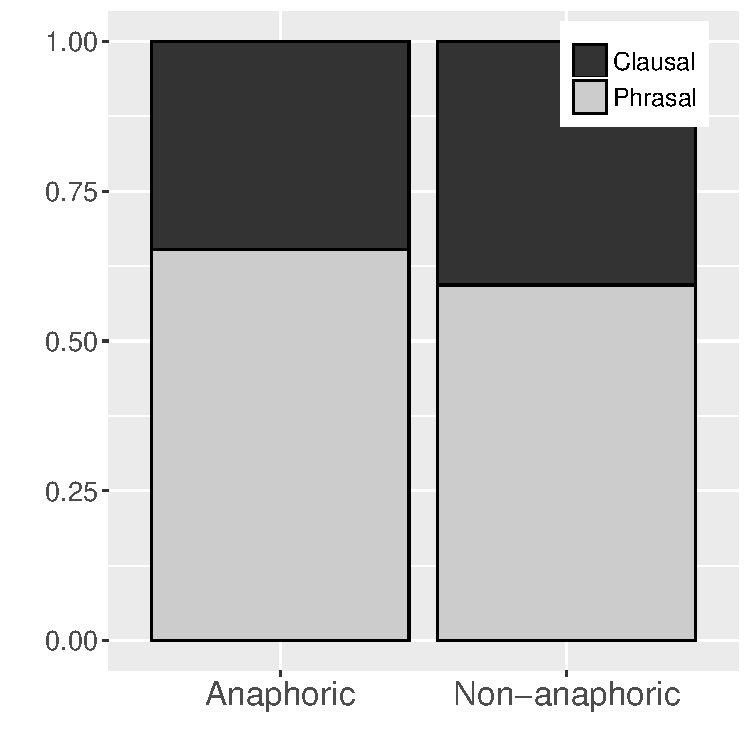
\includegraphics[width=.5\textwidth]{figure/IUInfoStatus.pdf}
	\caption{IU vs.~information status}
	\label{IUInfoStatusF}
	\end{center}
%\end{minipage}
\end{figure}
\begin{figure}
%\begin{minipage}{0.5\textwidth}
	\begin{center}
	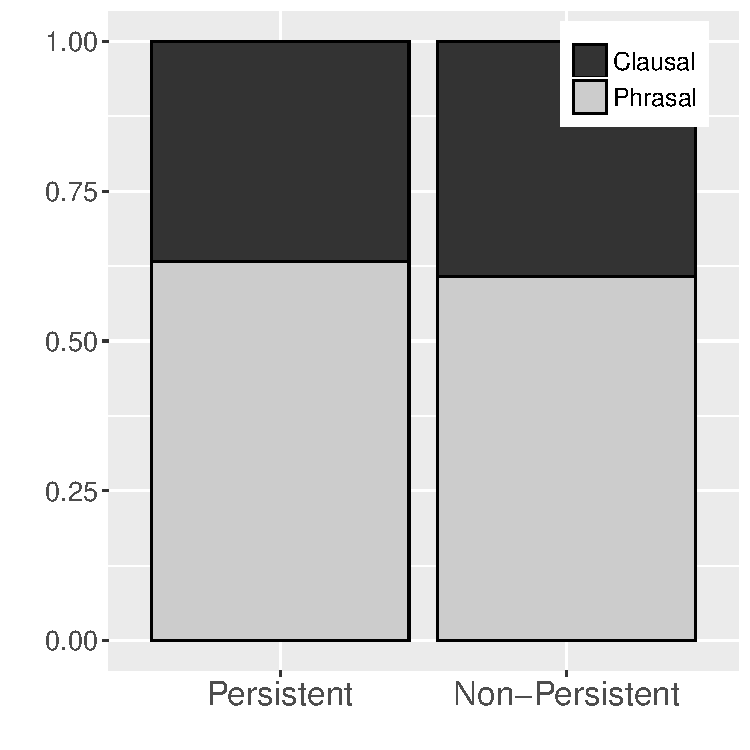
\includegraphics[width=.5\textwidth]{figure/IUPer.pdf}
	\caption{IU vs.~persistence}
	\label{IUPerF}
	\end{center}
%\end{minipage}
\end{figure}


%Since there are expected to be many factors affecting the distinction between phrasal vs.\ \isi{clausal} IU,
%I conducted logistic regression analysis using R.
%Table \ref{IntonationGlmT} shows the results of the analysis,
%where the dependent variable is the distinction between phrasal (\code{1}) vs.\ \isi{clausal} (\code{0}) IUs, and
%the independent variables are the following.
%%
%%\ex.
%% \a. Information Status: \isi{anaphoric} (\code{1}) and non-\isi{anaphoric} (\code{0})
%% \b. Persistence: persistent (\code{1}) and non-persistent (\code{0})
%% \b. Topic markers: \code{toiuno-wa}, \code{wa}, and \code{mo}
%% \b. grammatical function: \code{A}, \code{S}, \code{P}, and \code{LOC}
%% \b. Word order: \code{1}, \code{2}, \code{3}, and \code{4}
%
%\code{A} in \Last[d] indicates the \isi{agent-like argument} of a \isi{transitive clause},
%\code{S} indicates the only argument of an \isi{intransitive} clause,
%\code{P} indicates the patient-like argument of a \isi{transitive clause}, and
%\code{LOC} indicates locative, or elements potentially coded by \ci{ni}.%
%	\footnote{
%	As discussed earlier, both dative and locative are coded by the same form \ci{ni} in Japanese.
%	In this paper, I do not distinguish between dative and locative
%	and call them together locatives.
%	}
%The numbers in \Last[e] represent the order of arguments (A, S, P, and locatives).
%\code{1} indicates that the argument appears in the initial position,
%\code{2} indicates that it appears in the second position, and so on.
%Those variables whose p-values are more than $0.1$ are not shown in table \ref{IntonationGlmT}.
%
%I will discuss the relation between the dependent variable and each independent variable in the following sections.

This section explores the associations between IUs and \isi{information structure} by investigating our corpus.
I will argue that, in general, topics tend to be uttered in phrasal IUs (\S \ref{Int:IUISUnitCorp:Topic}),
while foci tend to be produced in \isi{clausal} IUs (\S \ref{Int:IUISUnitCorp:Focus}).
I also discuss exceptional cases for each tendency.

\chd{Table \ref{IUInfoStatusT} and Figure \ref{IUInfoStatusF} show the distribution of phrasal vs.~\isi{clausal} IUs
in different information statuses (\isi{anaphoric} vs.~non-\isi{anaphoric}).
Anaphoric elements refer to those whose referents have been mentioned in the previous \isi{discourse},
whereas non-\isi{anaphoric} elements refer to those whose referents have newly been mentioned
(see \ref{FW:Cor:TopFoc} for the annotation procedure more in detail).
A linear mixed effects model was employed to predict \isi{information status}, as we have seen in \S \ref{TopPar} and \S \ref{WO:Intro}.
Intonation (phrasal vs.~\isi{clausal} IU), particles (\ci{toiuno-wa, wa, mo, ga, o, ni}), and \isi{word order} (\code{nth} in CSJ, see \S \ref{WO:Intro} for the definition of this annotation) are included as fixed effects, and
the speaker (\code{TalkID} in the corpus) is included as a random effect.
The model with the effects of intonation, particles, and \isi{word order} is significantly different from that without each of them (likelihood ratio test, $p<0.05$ without intonation, $p<0.001$ a model without particles, and $p<0.01$ that without \isi{word order}).
}

\chd{
Table \ref{IUPerT} and Figure \ref{IUPerF} show the distribution of phrasal vs.~\isi{clausal} IUs in terms of persistence
(persistent vs.~non-persistent).
Persistent elements are those whose referents are to be mentioned again in the following \isi{discourse},
whereas non-persistent elements are those whose referents are not to be mentioned.
Again a linear mixed effects model was applied to predict persistence, as discussed in \S \ref{TopPar} and \S \ref{WO:Intro}.
Intonation, particles, and \isi{word order} are included as fixed effects and
the speaker as a random effect.
The model with the effects of particles, \isi{word order}, and intonation is not significantly different from that without the effect of intonation ($p=0.423$), whereas
it is significantly different from the model without each of the effects of particles and \isi{word order} (likelihood ratio test, $p<0.001$ a model without particles, $p<0.01$ that without \isi{word order}).
}

%%----------------------------------------------------
\subsection{Topics tend to be uttered in phrasal IUs}\label{Int:IUISUnitCorp:Topic}

This section and the next section
discuss associations between topics and IUs and
argue that
evoked, \isi{inferable}, declining and unused topics tend to be uttered in phrasal IUs (\S \ref{Int:Cor:Topic:PIU}, \ref{Int:Cor:InacTopic:PIU}).
I also claim that some strongly evoked topics, especially pronouns, are in fact part of the following IU
and should be counted as \isi{clausal} IUs
by modifying the definitions of IU (\S \ref{Int:Cor:Topic:CIU}).
It also discusses exceptional cases where topics appear in \isi{clausal} IUs (\S \ref{TopCIU}).
I will argue that topics to be established tend to be uttered in phrasal IUs (\S \ref{Int:Disc}).
%Finally, it proposes principles that operates IUs and
%argues that

\begin{table}
 \centering
 \tblcaption{Intonation unit vs.~particles}
 \label{IUParT}
\begin{tabular}{lrrrrrr}
 \toprule
            & \ci{toiuno-wa} & \ci{wa}       & \ci{mo}       & \ci{ga}       & \ci{o}        & \ci{ni} \\
 \midrule
 Phrasal IU &  64            & 157           &  81           &   270         &  160          & 259  \\
            & \rt{(95.5\%)} & \rt{(83.5\%)}  & \rt{(68.6\%)} & \rt{(60.0\%)} & \rt{(47.1\%)} & \rt{(58.6\%)} \\
 Clausal IU &  3             & 31            &  37           & 180           &  180           & 183  \\ 
            & \rt{(4.5\%)}   & \rt{(16.5\%)} & \rt{(31.4\%)} & \rt{(40.0\%)} & \rt{(52.9\%)} & \rt{(41.4\%)} \\
 \midrule
 Sum        &  67            &  188          &  118          &   450         &  340          &  442 \\
            & \rt{(100\%)}   & \rt{(100\%)} & \rt{(100\%)}   & \rt{(100\%)}  & \rt{(100\%)} & \rt{(100\%)} \\
 \bottomrule
\end{tabular}
\end{table}

\begin{figure}
	\begin{center}
	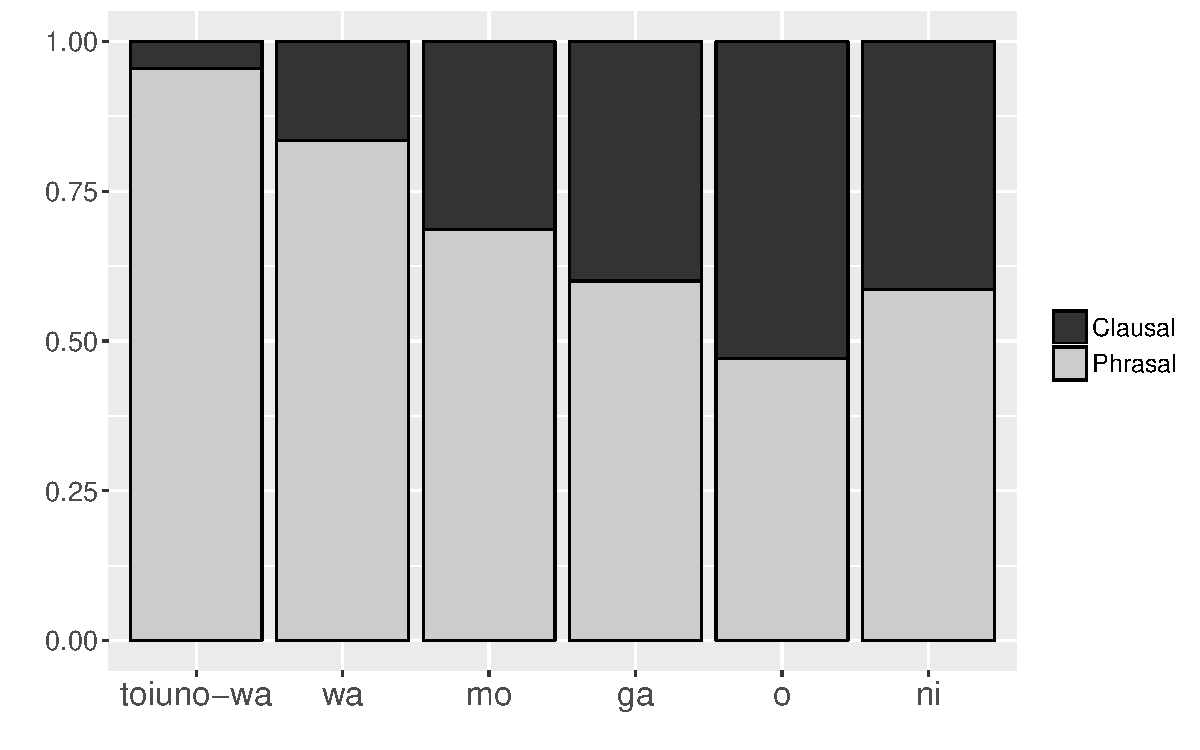
\includegraphics[width=.7\textwidth]{figure/IUPar.pdf}
	\caption{Intonation unit vs.~particles}
	\label{IUParF}
	\end{center}
\end{figure}


%%----------------------------------------------------
\subsubsection{Evoked, inferable, and declining elements with topic markers in phrasal IUs}\label{Int:Cor:Topic:PIU}

As Table \ref{IUInfoStatusT}, Figure \ref{IUInfoStatusF}, and the results of statistical analysis indicate,
%the existence of \isi{topic} markers is a feature that significantly affects the distinction between phrasal vs.\ \isi{clausal} IUs;
\isi{anaphoric} elements are more likely to be uttered in phrasal IUs.
Also, Table \ref{IUParT} and Figure \ref{IUParF} show that
elements with \isi{topic} markers such as \ci{toiuno-wa} and \ci{wa} are more likely to be in phrasal IUs than those with case markers.
Elements with \isi{topic} markers are uttered in phrasal IUs most of the time,
while the ratio of elements with case markers (without \isi{topic} markers) in \isi{clausal} IUs is larger.
These observations indicate that
at least evoked and \isi{inferable} topics tend to be produced in phrasal IUs.
This conclusion results from the observation that
elements coded by \isi{topic} markers such as \ci{toiuno-wa} and \ci{wa}
are evoked or \isi{inferable} elements as argued for in Chapter \ref{Particles}.
Below I show that declining elements are also uttered in phrasal IUs.
I will argue that strongly evoked elements, especially pronouns, are in fact part of the following IUs,
although in the current criteria they are included in phrasal IUs,
and should be counted as phrasal IUs in \S \ref{Int:Cor:Topic:CIU}.

%Note that the existence of \isi{topic} markers significantly contribute to the distinction between phrasal vs.\ \isi{clausal} IUs
%controlling other variables such as \isi{word order}.
%As shown in Chapter \ref{WordOrder},
%elements with \isi{topic} markers tend to appear clause-initially.
%One might claim that clause-initial elements are more likely to be uttered in phrasal IUs because the distance between the element and the predicate is larger.
%However, the result is obtained taking \isi{word order} into consideration.
%Therefore this claim does not hold.
%
\begin{figure}
%\begin{minipage}{0.5\textwidth}
	\begin{center}
	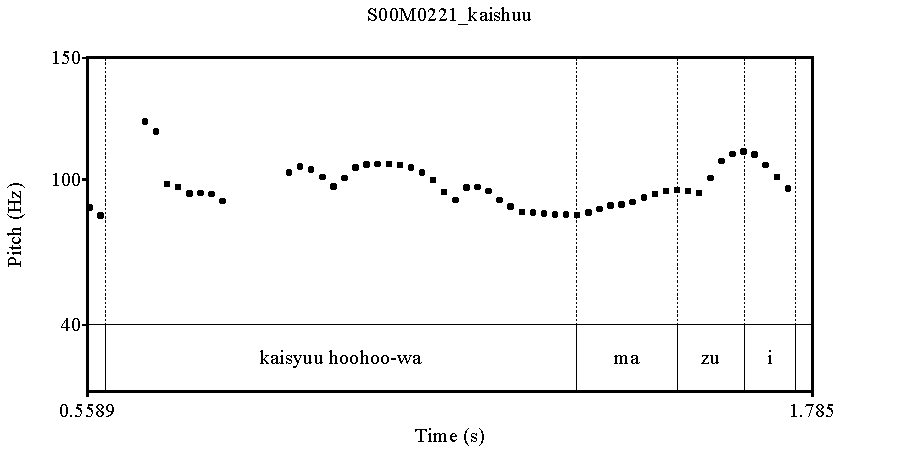
\includegraphics[width=.5\textwidth]{sounds/S00M0221_kaishuu.pdf}
	\caption{Pitch contour of \ref{S00M0221_kaishuu}}
	\label{S00M0221_kaishuuF}
	\end{center}
%\end{minipage}
\end{figure}
\begin{figure}
%\begin{minipage}{0.5\textwidth}
	\begin{center}
	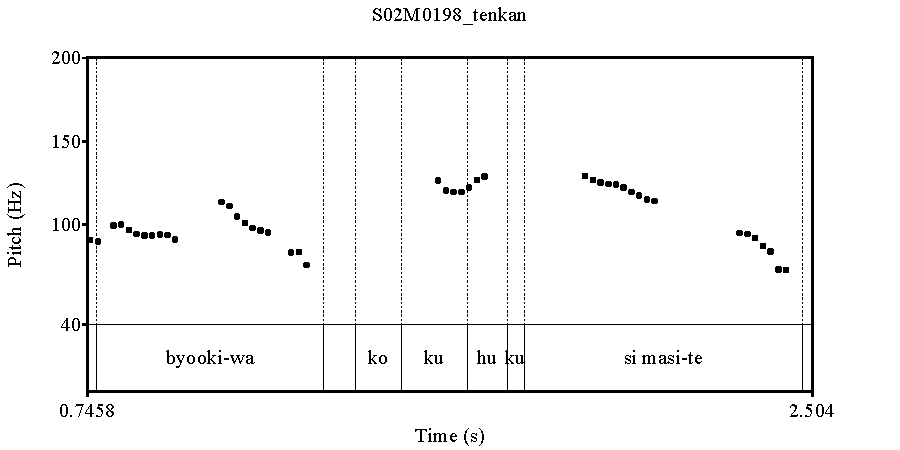
\includegraphics[width=.5\textwidth]{sounds/S02M0198_tenkan.pdf}
	\caption{Pitch contour of \ref{S02M0198_tenkan}}
	\label{S02M0198_tenkanF}
	\end{center}
%\end{minipage}
\end{figure}
\begin{figure}
%\begin{minipage}{0.5\textwidth}
	\begin{center}
	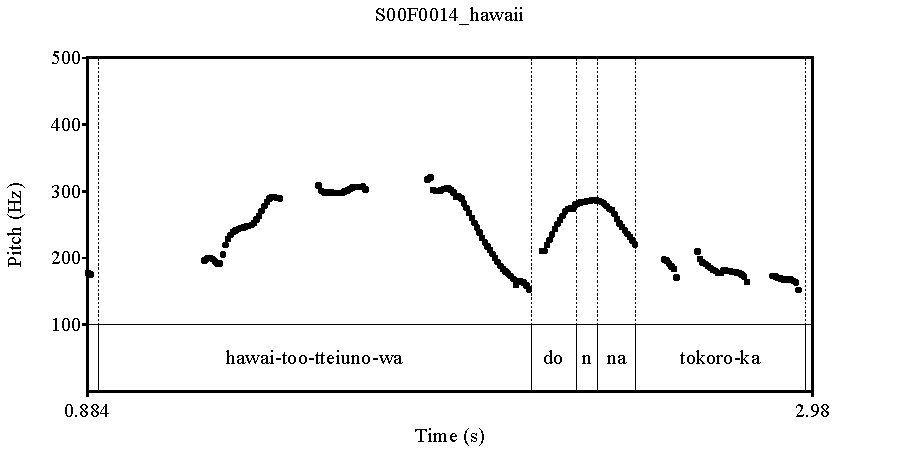
\includegraphics[width=.5\textwidth]{sounds/S00F0014_hawaii.pdf}
	\caption{Pitch contour of \ref{S00F0014_hawaii}}
	\label{S00F0014_hawaiiF}
	\end{center}
%\end{minipage}
\end{figure}
\begin{figure}
%\begin{minipage}{0.5\textwidth}
	\begin{center}
	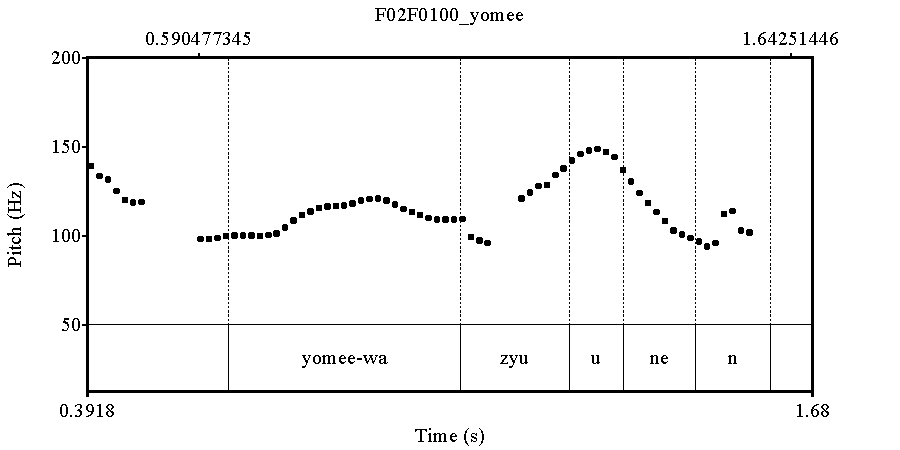
\includegraphics[width=.5\textwidth]{sounds/s02F0100_yomee.pdf}
	\caption{Pitch contour of \ref{S02F0100_yomee}}
	\label{S02F0100_yomeeF}
	\end{center}
%\end{minipage}
\end{figure}

\Next exemplifies an evoked element with \isi{topic} marker
uttered in a phrasal IU
(``\tp{\dvline}'' indicates IU boundaries).
In this talk, the speaker is talking about his former job,
collecting debt from people.
There is an IU boundary after \ci{kaisyuu hoohoo-wa} `collecting method-\ci{wa}', the element coded by a \isi{topic} marker.
\ci{kaisyuu hoohoo} `collecting method' is evoked because
it is mentioned in the immediate context
as indicated by \ci{koo it-ta} `this way of'.
%
\exg.\label{S00M0221_kaishuu}koo it-ta \tp{\dvline} \EM{kaisyuu} \EM{hoohoo-wa} \tp{\dvline} \EMi{mazui}-to \tp{\dvline} \\
	this.way say-\ab{past} {} collecting method-\ci{wa} {} wrong-\ab{quot} {} \\
	`This way of collecting (debt) is wrong...'
	\src{S00M0221: 580.21-582.06}
%S00M0221|00574657L|574.656905|595.534525|L|んで(0.193)新聞にも商工ローンの見出しがたくさん載って(0.89)(F お)(0.177)こういった回収方法はまずいと(0.764)(F おー)(F んー)もっと(D うー)(1.04)回収倫理規定に法に則って(0.179)(F えー)仕事をしなさいということを(1.654)(F えー)(0.756)会社の方から(0.472)強く言われまして|/テ節/|

Figure \ref{S00M0221_kaishuuF} shows the \isi{pitch contour} of \Last.
In the figure,
one can observe a \isi{pitch reset} in the \isi{first mora} of the predicate \ci{mazui} `wrong'.

\Next is another example,
where the speaker is talking about his dog,
who had epilepsy.
There is an IU boundary after \ci{byooki-wa} `disease-\ci{wa}'.
\ci{Byooki} `disesase' is also evoked because it is mentioned in the immediate context
as indicated by the \isi{demonstrative} \ci{sono} `that'.
%
\exg.\label{S02M0198_tenkan}sono \EM{byooki-wa} \tp{\dvline} {kokuhuku} \EMi{si}-masi-te \tp{\dvline} \\
		that disease-\ci{wa} {} overcome do-\ab{plt}-and {} \\
		`(The speaker's dog) overcame that disease.'
		\src{S02M0198: 480.52-482.47}
%S02M0198|00476548L|476.547845|484.196228|L|(F まー)幸いなことに(0.106)(F そのー)(0.81)てんかん(0.277)と言うか(F ま)その病気は克服しまして(0.579)治ったんですが|/並列節ガ/|

The \isi{pitch contour} of \Last is shown in Figure \ref{S02M0198_tenkanF}.
In the figure,
one can observe not only a \isi{pitch reset},
but also \isi{falling intonation},
which typically occurs IU-finally.

\Next is an example of \ci{toiuno-wa}-coded element uttered in a phrasal IU.
The \isi{pitch contour} is shown in Figure \ref{S00F0014_hawaiiF}.
\ci{Hawai-too} `Hawaii island' is also evoked
as is clear from the \isi{demonstrative} \ci{kono} `this'.
%
\exg.\label{S00F0014_hawaii}de kono \tp{\dvline} \EM{hawai-too-tteiuno-wa} \tp{\dvline} don'na \EMi{tokoro}-ka-tte ii-masu-to \tp{\dvline} \\
		then this {} Hawaii-island-\ci{toiuno}-\ci{wa} {} how place-\ab{q} say-\ab{plt}-\ab{cond} {} \\
		`What kind of place is this Hawaii island?'
		\src{S00F0014: 166.53-169.71}
%S00F0014|00166531L|166.531125|169.714444|L|でこの(0.268)ハワイ島っていうのはどんなところかって言いますと|/条件節ト/|

As shown in the figure,
one can observe the \isi{pitch reset} in the \isi{first mora} of the predicate \ci{don'na} `how'.

Similarly,
the \isi{inferable} element \ci{yomee-wa} `life.expectancy-\ci{wa}' is produced in a phrasal IU as indicated in Figure \ref{S02F0100_yomeeF}.
\ci{Yomee} `life.expectancy' is \isi{inferable}
because the speaker is talking about her disease and
it is reasonable to assume that life expectancy is part of the knowledge about disease.
%
\exg.\label{S02F0100_yomee}osoraku {\iub} \EM{yomee-wa} {\iub} \EMi{zyuu-nen} {\iub} -da-to {\iub} iwa-re-masi-ta \\
      probably {} life.expectancy-\ci{wa} {} ten-\ab{cl}.year {} -\ab{cop}-\ab{quot} {} say-\ab{pass}-\ab{plt}-\ab{past} \\
      `(I) was told that (my) life expectancy was 10 years.'
      \src{S02F0010: 312.22-314.91}
%S02F0100|00300638L|300.637726|314.908404|L|その治療法というのは唯一(0.33)私が使うことのできないステロイド剤で進行遅らせる(0.344)ことだけで(1.347)(D そよ)(0.154)(F その)進行遅らせた状態で(0.17)恐らく余命は十年(0.35)だと言われました|[文末]|


Declining elements are also produced in phrasal IUs rather than \isi{clausal} IUs.
Consider the following example.
In \Next,
two competing topics, \ci{meisei} `fame' and \ci{sigoto} `job',
are introduced in line a.
Then, the speaker starts to talk about fame first and moves onto `job' in line g,
where the \isi{topic} \ci{sigoto} `job' is considered to be declining.
In this case, there is an intonation-unit boundary after \ci{sigoto-no bubun-na-n-desu-keredomo} `concerning the other one, job'.
%
\ex.
 \a. I have two goals: one is for \EMi{fame} and the other is for \EMi{\EMi{job}}.
 \b. Concerning \EMi{fame},
 \b. I have been participating in various \isi{piano} competitions
 \b. So far the best award I received was the fourth best place in the China-Japan International Competition.
 \b. Beyond that, I would like to receive higher awards.
 \b. Titles matter a lot for pianists, so I will work hard.
 \bg. de {\iub} ato-wa {\iub} \EM{sigoto-no} {\iub} \EM{bubun-na-n-desu-keredomo} {\iub} \\
 	then {} remaining-\ci{wa} {} job-\ab{gen} {} part-\ab{cop}-\ab{nmlz}-\ab{cop}.\ab{plt}-though {} \\
	`Concerning the other one, job,'
 \b. to receive higher wages...
\hfill{(\code{S00F0209: 495.77-539.19})}
%
%これからのあの目標っていうのがありまして
%まそれは大きく分けて二つあるんですけども
%ま名声の部分と仕事っていう部分がありまして
%一番目の名声の部分は
%やはりあの今まで受けたコンクールの最高順位が
%あのま日中友好国際音音楽コンクールっていうのがあって
%それがまー一般のピアノ部門で四位で奨励賞だったんですね
%でそれを超えてあの三位以内に入賞することがまず一つで
%あのどうしてもこれはやっぱりピアノを志す者にとっては
%このタイトルってのは凄く大きいので
%あのやってきたいです
%で後は仕事の部分なんですけれども
%あの一回のギャランティーがえーと勿論アップするように
% (S00F0209: 495.77-539.19)


%\Next exemplifies \ci{mo}-coded elements uttered in a phrasal IU
%and Figure \ref{S01F0038_yumeF} shows the \isi{pitch contour} of the example.
%%
%\exg.\label{S01F0038_yume}anoo kekkyoku \tp{\dvline} ee ma bareebooru-sensyu-no \EM{yume-mo} \tp{\dvline} dan'nen itasi-masi-te \tp{\dvline} \\
%	\ab{fl} eventually {} \ab{fl} \ab{fl} volleyball-player-\ab{gen} dream-also {} give.up do.\ab{hbl}-\ab{plt}-and {} \\
%	`Eventually (I) gave up my dream of (becoming) a volleyball player.'
%	\src{S01F0038: 83.61-87.81}
%%S01F0038|00083609L|83.609345|87.812375|L|(F あのー)結局(0.119)(F えー)(F ま)バレーボール選手の夢も断念いたしまして|/テ節/|
%
%Like other examples of \isi{topic} markers,
%one can observe a \isi{pitch reset} after the \isi{topic} marker \ci{mo}.


%%----------------------------------------------------
\subsubsection{Unused elements with topic markers in phrasal IUs}\label{Int:Cor:InacTopic:PIU}

Unused elements with \isi{topic} markers also tend to be uttered in
phrasal IUs.
Elements coded by a \isi{copula} plus \ci{kedo} or \ci{ga} appear
in phrasal IUs most of the time.
For example, in \Next[a],
the element \ci{sutairu} `style', which is introduced for the first time,
are produced in a phrasal IU.%
	\footnote{
	In fact, the predicate of `style' is not clear in this example.
	This is a general characteristics of topics.
	See discussion in \S \ref{Par:Subj:Ex} for more detail.
	}
%
\ex.
 \ag. nde {\iub} ee {\iub} kono {\iub} tabi-no {\iub} \EM{sutairu} {\iub} \EM{-tteiu} \EM{mono-na-n-desu-keredomo} {\iub} \\
      and {} \ab{fl} {} this {} travel-\ab{gen} {} style {} -\ci{toiu} thing-\ab{cop}-\ab{nmlz}-\ab{cop}.\ab{plt}-though \\
      `Regarding my style of travelling,'
 \b. uh, I'm kind of getting used to travelling,
 \b. uh, I want to travel cheaply and
 \b. go anywhere freely by myself,
 \b. that was my style of travelling, so...
     \src{S00F0014: 300.43-317.95}
%S00F0014|00300431L|300.430603|306.188251|L|んで(0.512)(F えー)(0.932)この(0.789)旅のスタイル(0.542)っていうものなんですけれども|/並列節ケレドモ/|
%S00F0014|00306553L|306.552902|317.951795|L|(F あのー)私はもう結構(0.111)(F ま)(0.164)旅慣れてると言うか(0.269)(F あの)(0.119)とにかく安くて自分で自由に(0.312)色んなとこ行きたいっていうのが(0.296)ずっと(F その)自分の旅のスタイルだったものですから|<理由節カラ>|話題導入表現

Similarly,
in \Next[a],
\ci{kandoo} `emotion' is mentioned for the first time and
is produced in a phrasal IU.
%
\ex.
 \ag. de eberesuto-o mi-ta \EM{kandoo-na-n-desu-keredomo} {\iub} \\
      and Everest-\ci{o} see-\ab{past} emotion-\ab{cop}-\ab{nmlz}-\ab{cop}.\ab{plt}-though {} \\
      `Talking about the emotion of seeing Everest,'
 \b. um, Himalaya Mountains have a very unique shape I've never seen before,
 \b. Actually, local people call them holy mountains,
 \b. hm, somehow their shapes are sacred.
     \src{S01F0151: 460.73-477.82}
%S01F0151|00460734L|460.734005|462.737112|L|でエベレストを見た感動なんですけれども|/並列節ケレドモ/|
%S01F0151|00463340L|463.340088|477.823907|L|(F えー)ヒマラヤの山々っていうのは(0.265)今までに見たことがないぐらい非常に特徴的な形をした山が多くてですね(0.334)実際に現地の方々は(0.24)聖なる山(0.162)って呼んでいる山が非常に多いぐらい(0.394)(F まー)何か近付き難いような山の形をしておりました|[文末]|


Readers might speculate that
these elements appear in phrasal IUs because they are long expressions.
However, examples of the experimental study in \S \ref{Int:IUISUnitExp} that force the speakers to assume topics to be unused,
are short expressions (one word).
The experiment show that
these short unused topics are still produced in phrasal IUs.


%%----------------------------------------------------
\subsubsection{Strongly evoked elements in clausal IUs}\label{Int:Cor:Topic:CIU}

\begin{figure}
%\begin{minipage}{0.5\textwidth}
	\begin{center}
	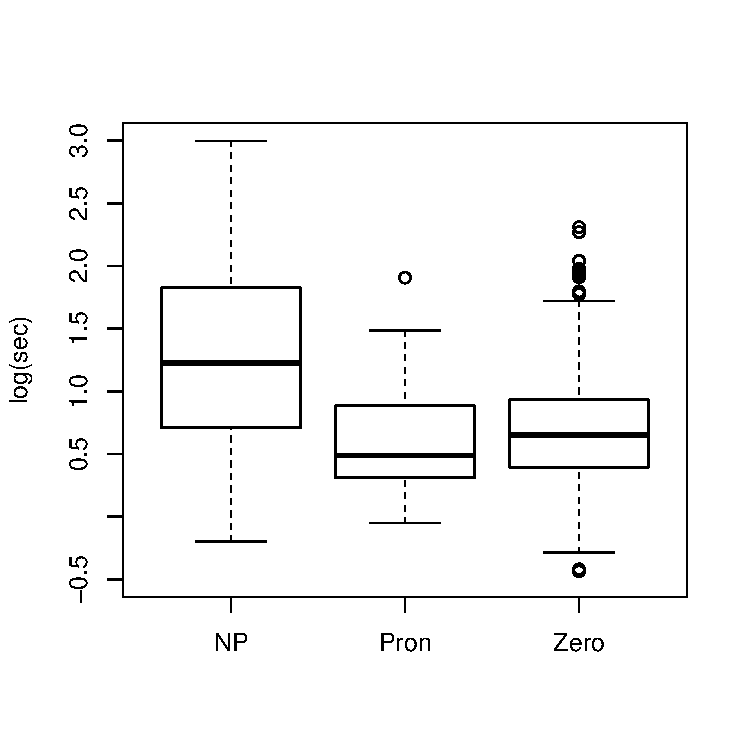
\includegraphics[width=0.6\textwidth]{figure/DistExpType.pdf}
	\caption{Anaphoric distance vs.\ expression type (all)}
	\label{DistExpTypeF3}
	\end{center}
%\end{minipage}
%\begin{minipage}{0.5\textwidth}
%	\begin{center}
%	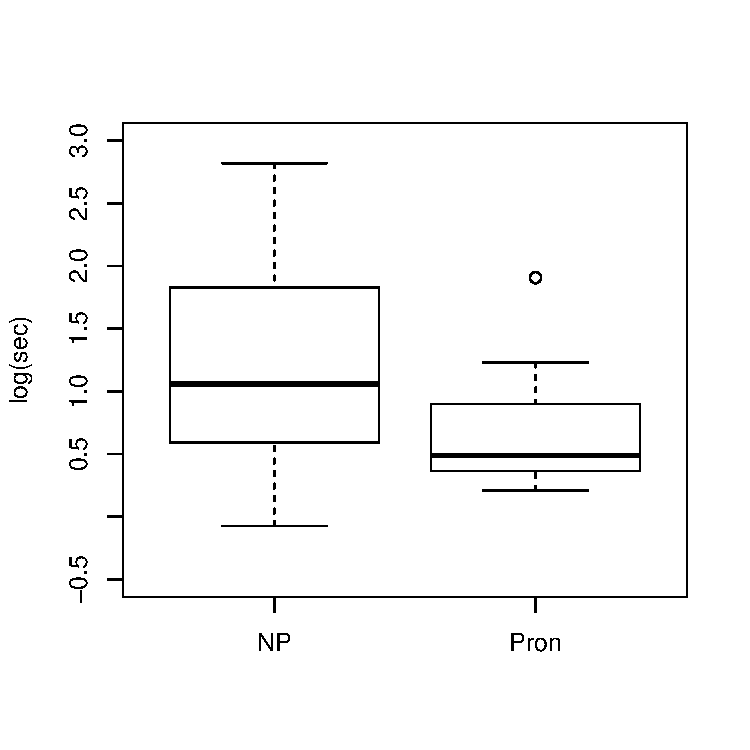
\includegraphics[width=0.99\textwidth]{figure/DistExpTypeTop.pdf}
%	\caption{Anaphoric distance vs.\ expression type (coded by topic markers)}
%	\label{DistExpTypeParF2}
%	\end{center}
%\end{minipage}
\end{figure}


I propose that strongly evoked elements, usually pronouns coded by \isi{topic} markers, are uttered in \isi{clausal} IUs,
although they are categorized into phrasal IUs by the current definition.
Because strongly evoked elements tend to be uttered in \isi{low pitch} with smaller \isi{pitch range} than the following \isi{accentual phrase},
they are likely to be counted as phrasal IUs.
However, I argue that they should be regarded as \isi{clausal} IUs.
The number of pronouns are very small, which does not influence the overall tendency in Figure \ref{IUParF} and Table \ref{IUParT} and
hence this change does not affect the conclusion proposed in the last section.
The claim that pronouns are strongly evoked elements
is supported in
Figure \ref{DistExpTypeF3},
repeated from Figure \ref{DistExpTypeF2},
which shows the time difference between
when the \isi{first mora} of the element in question is produced and
when that of its \isi{antecedent} is produced.
%Zero pronouns are tantatively supposed to be produed at the time when
%the predicate starts to be produced.
This is assumed to approximate the \isi{activation cost} of elements.
As indicated in the figure,
pronouns have as \isi{low activation} costs as zero pronouns.

First, I show examples of strongly evoked elements and their \isi{pitch} contours.
The \isi{pitch} contours are different from evoked elements we have seen
in the previous section.
\Next is one of the few examples from the corpus of the current study, CSJ,
whose \isi{pitch contour} is shown in Figure \ref{S00F0014_soreF}.
The IU boundary ``\iub'' is inserted based on the current definition.
I argue that there is no boundary after \ci{sore-wa} `that-\ci{wa}'.
%
\exg.\label{S00F0014_sore}\EM{sore-wa} \tp{\dvline} \EMi{nan}-daroo-to omot-te \tp{\dvline} \\
		that-\ci{wa} {} what-\ab{cop}.\ab{infr}-\ab{quot} think-and {} \\
		`(I) was wondering what it was...'
		\src{S00F0014: 654.06-655.18}
%それは何だろうと思って

Since the number of pronouns is small in the current corpus,
I provide examples from another corpus.
Examples \Next and \NNext are from
\ci{the Chiba three-party conversation corpus},
which is a corpus of three people's casual conversation \cite{Den_2007_SAC}.
Their \isi{pitch} contours are shown in Figures \ref{chiba0232_areF} and \ref{chiba1232_soreF} respectively.
Again, the IU boundary is inserted based on the current definition
that I challenge.
%
\exg.\label{chiba0232_are}\EM{are} \tp{\dvline} \EMi{kir}-en-no-ka-na \tp{\dvline} \\
		that {} cut-\ab{cap}-\ab{nmlz}-\ab{q}-\ab{q} {} \\
		`Can (you) cut it?'
		\src{chiba0232: 442.56-443.33}

\exg. \label{chiba1232_sore}\EM{sore} \tp{\dvline} \EMi{dame}-zyan \tp{\dvline} \\
		that {} wrong-\ab{fp} {} \\
		`It's wrong, isn't it?'
		\src{chiba1232: 155.92-156.64}
%\exg. dakara are kin-nai-to ike-nai \\
%		so that cut-\ab{neg}-\ab{cond} go-\ab{neg} \\
%		`So, (you) have to cut it.'
%		\src{chiba0232: 441.41-442.27}

As shown in Figure \ref{S00F0014_soreF}-\ref{chiba1232_soreF},
there is neither a pause nor \isi{vowel} lengthening,
which is often observed IU-finally.
Moreover, the accent nucleus is not clearly observed in these pronouns.
This suggests that
a phrasal IU of evoked elements coded by \isi{topic} markers and
that of strongly evoked elements are qualitatively different.
Since strongly evoked elements are already evoked and do not need to attract the \isi{hearer}'s attention,
they are uttered with lower \isi{pitch}.
When they are followed by the predicate, which is typically not evoked and needs to attract the \isi{hearer}'s attention,
the predicate is uttered with higher \isi{pitch},
which causes a \isi{pitch reset}.
%\citeA{nakagawaden12slud}, who studied the relation between \isi{information structure} and IU in dialogues using the same criteria of identifying IUs,
%found an effect of \isi{pronoun} (as opposed to full noun phrase) contributing to the status of phrasal IUs.


%The F$_{0}$ peak of the pronouns \ci{are} and \ci{sore} in these figures
%are lower than that of the following predicate.
%This is because they are \isi{anaphoric} elements.
%Anaphoric elements pronounced in low F$_{0}$ have been reported in many languages including
%Japanese \cite[Chapter 6]{venditti00}
%\ili{Dutch} \cite{vandonzeletal97,swertsetal02},
%\ili{German} \cite{ferykugler08,baumanriester13},
%Swedish \cite{bruce77}, and
%\ili{English} \cite{halliday67_\isi{pitch},halliday67,bolinger72,chafe76,brown83,terken84}.
%%%% そうでない言語もある: インド・カリブの英語、ハワイのピジン (Vanderslice and Pierson, 1967; Gumperz, 1982: ch.5)
%The fact that this phenomenon is not unique to Japanese but is observed cross-linguistically
%supports the explanation that lower F$_{0}$ on \isi{anaphoric} elements is motivated by human cognition or some other factors shared by all human beings;
%because the speaker needs to pronounce non-\isi{anaphoric} elements with more prominence than \isi{anaphoric} elements to attract the \isi{hearer}'s attention to the non-\isi{anaphoric} elements,
%F$_{0}$ of \isi{anaphoric} elements are lower than that of non-\isi{anaphoric} elements.
%If this phenomenon is not cognitively motivated,
%the selection must be random, i.e.,
%it is predicted that,
%in some languages, speakers produce \isi{anaphoric} elements with high F$_{0}$ and non-\isi{anaphoric} elements with low F$_{0}$,
%while, in other languages, speakers do vice versa.
%However, this is not the case.
%Many languages seem to have the same tendency.
%This universal tendency that \isi{anaphoric} elements are pronounced in lower F$_{0}$ than non-\isi{anaphoric} elements and the fact that they tend to be produced before non-\isi{anaphoric} elements, which typically include predicates, explain why there tend to be IU boundaries after \isi{anaphoric} elements, i.e., they tend to be uttered in phrasal IUs.

I challenge the claim that this type of strongly evoked element actually forms a single chunk of processing.
First,
in addition to the qualitative difference between phrasal IUs of evoked elements and of strongly evoked elements,
the transition from the IU with a single strongly evoked element such as \ci{are} and \ci{sore} in Figure \ref{S00F0014_soreF}-\ref{chiba1232_soreF} to the next is too fast for the speaker to plan the next \isi{utterance},
assuming that an IU represents some kind of processing unit.
This suggests that the current element and the following element(s) belong to a single processing unit.

Second, a single strongly evoked element is too small a number for a processing unit.
Pronouns in particular are of relatively high frequency (although they are less frequent than zero pronouns) and the referent is assumed to have been evoked both in the speaker's and the \isi{hearer}'s mind.
Although ``the magic number'' is still controversial (including the skepticism about ``expressing capacity limits of human cognition in terms of a number'' \cite[][p.~245]{oberauer07}),
\citeA{cowan00,cowan05} estimates that the magic number is around four in healthy young adults,
whereas, in the original proposal in \citeA{miller56},
the number is seven plus or minus two.
Anyway, one element is too small in terms of this magic number.


%Third,
%when \isi{anaphoric} elements are contrasted,
%they have 

Third,
it is known that, historically, unstressed pronouns can change into clitics, then into affixes \cite{givon76}.
Japanese pronouns such as \ci{are} and \ci{sore} are not exceptions;
\ci{r} in \ci{are} and \ci{sore} are sometimes reduced and are uttered very quickly,
which is highly likely to become a motivation for them to change into clitics in the future.
Moreover, these pronouns often do not seem to have a clear \isi{pitch peak} any more.
The original \isi{pitch accent} of \ci{kore}, \ci{sore}, and \ci{are} is LH
(The accent type of \ci{kore}, \ci{sore}, and \ci{are} is a flat type;
i.e., they do not have accent nucleus).
However, at least the \isi{pitch} contours of the pronouns in Figure \ref{S00F0014_soreF}-\ref{chiba1232_soreF} are not LH any more.%
	\footnote{
	This breaks one of the \isi{pitch accent} principles of Japanese discussed in \S \ref{BackSubSecGeneralChar},
	which states that the pitches of the first and the second morae within a word must be different.
	I claim that this is one of the motivations for pronouns to appear after the predicate.
	See also \S \ref{WO:PostP:Motivations:IU} for discussion.
	}
The \isi{pronoun} \ci{are} in Figure \ref{chiba0232_areF} is completely low,
and \ci{sore-wa} in Figure \ref{S00F0014_soreF} is HL, whose first \isi{pitch} I believe is high because the \isi{pronoun} appear utterance-initially.
When such \isi{clitic} pronouns start to phonologically depend on other words,
it becomes harder to argue that a single \isi{clitic} corresponds to a single processing unit.

From the observations above,
I propose that IUs with a single \isi{anaphoric element} do not form a single processing unit;
rather, it is more appropriate to integrate it to the following IU and regard the whole chunk as a unit of processing.
How to decide to integrate some IUs into the following IUs but not others is necessary to investigate in the future research.

%I argue that integrating strongly active elements (which are often topics) into the predicate IU and uttering a \isi{topic} in an IU and a focus in another IU are two different competing motivations \cite{dubois85}
%and the speaker decides which motivation to prefer.


\begin{figure}
%\begin{minipage}{0.5\textwidth}
	\begin{center}
	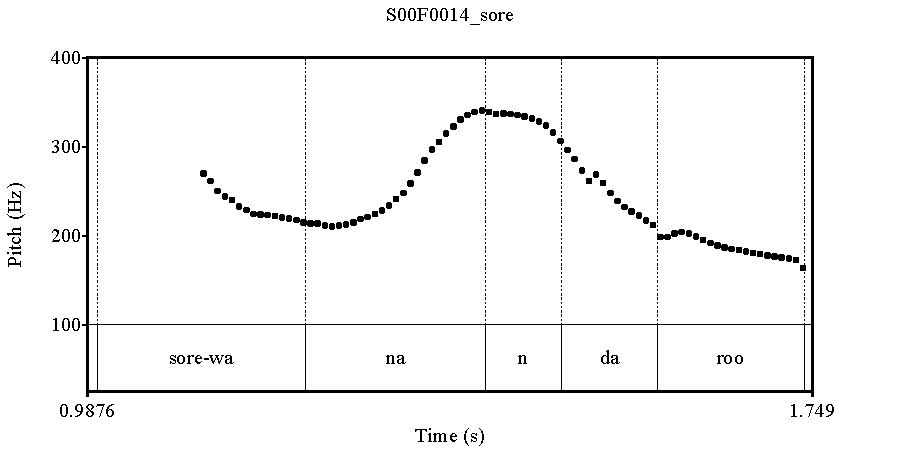
\includegraphics[width=.95\textwidth]{sounds/S00F0014_sore.pdf}
	\caption{Pitch contour of \ref{S00F0014_sore}}
	\label{S00F0014_soreF}
	\end{center}
%\end{minipage}
\end{figure}
\begin{figure}
%\begin{minipage}{0.5\textwidth}
	\begin{center}
	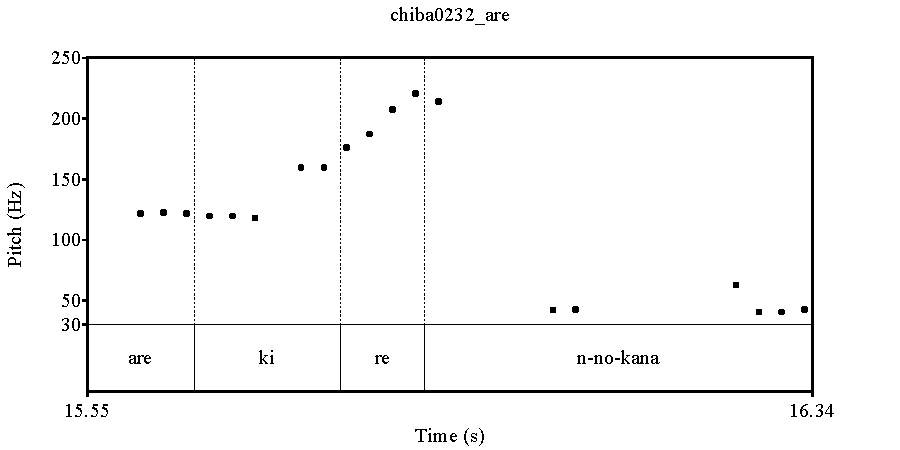
\includegraphics[width=.95\textwidth]{sounds/chiba0232_are.pdf}
	\caption{Pitch contour of \ref{chiba0232_are}}
	\label{chiba0232_areF}
	\end{center}
%\end{minipage}
\end{figure}
\begin{figure}
%\begin{minipage}{0.5\textwidth}
	\begin{center}
	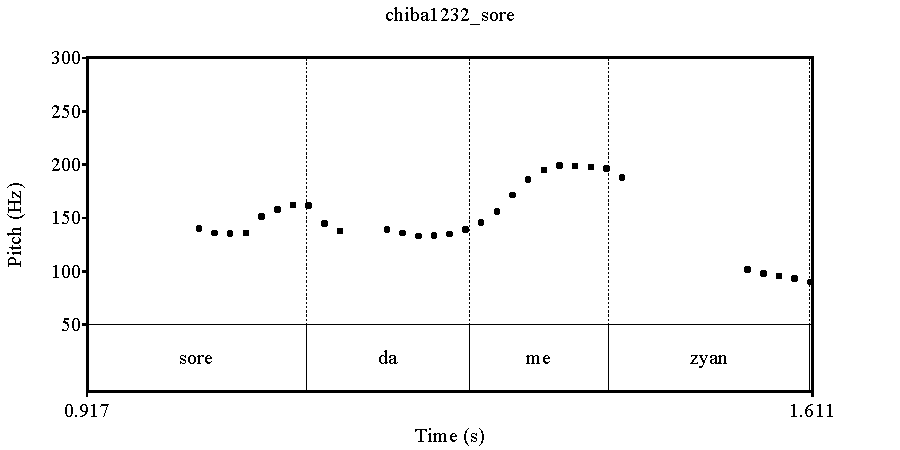
\includegraphics[width=.95\textwidth]{sounds/chiba1232_sore.pdf}
	\caption{Pitch contour of \ref{chiba1232_sore}}
	\label{chiba1232_soreF}
	\end{center}
%\end{minipage}
\end{figure}

%%%ISSUE The sizes of figures are different.


%%----------------------------------------------------
\subsubsection{Elements with topic markers in clausal IUs}\label{TopCIU}

\begin{figure}
%\begin{minipage}{0.5\textwidth}
	\begin{center}
	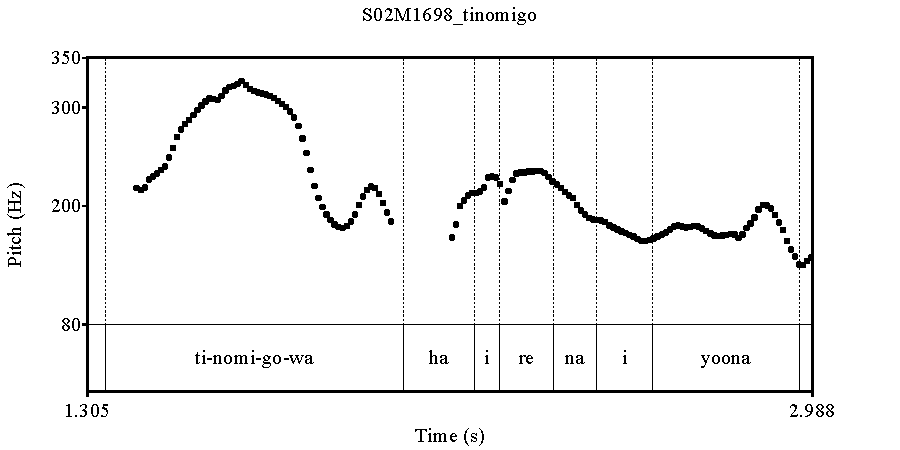
\includegraphics[width=.6\textwidth]{sounds/S02M1698_tinomigo.pdf}
	\caption{Pitch contour of a in \ref{S02M1698_tinomigo}}
	\label{S02M1698_tinomigoF}
	\end{center}
%\end{minipage}
\end{figure}
\begin{figure}
%\begin{minipage}{0.5\textwidth}
	\begin{center}
	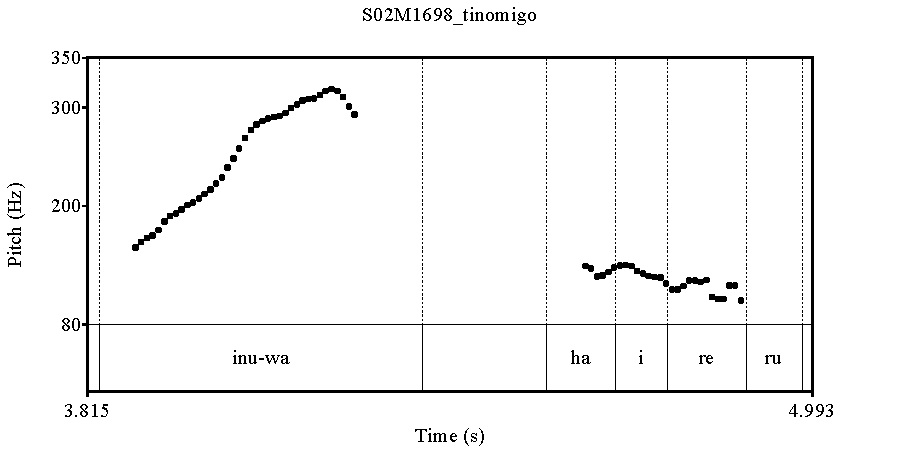
\includegraphics[width=.6\textwidth]{sounds/S02M1698_inu.pdf}
	\caption{Pitch contour of b in \ref{S02M1698_tinomigo}b}
	\label{S02M1698_inuF}
	\end{center}
%\end{minipage}
\end{figure}
\begin{figure}
%\begin{minipage}{0.5\textwidth}
	\begin{center}
	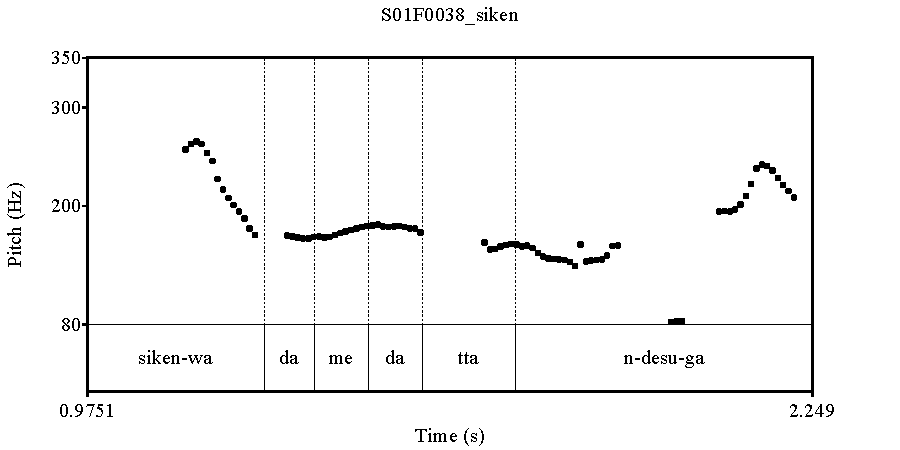
\includegraphics[width=.6\textwidth]{sounds/S01F0038_siken.pdf}
	\caption{Pitch contour of \ref{S01F0038_siken}}
	\label{S01F0038_sikenF}
	\end{center}
%\end{minipage}
\end{figure}

I have claimed that
evoked topics tend to be uttered in phrasal IUs,
while strongly evoked topics tend to be uttered in \isi{clausal} IUs.
This section discusses cases where
lexical NPs coded by \isi{topic} markers are produced in \isi{clausal} IUs
for several reasons.

First, contrasted elements coded by \isi{topic} markers are typically uttered in a \isi{clausal} IU;
the \isi{pitch range} of contrasted elements with the \isi{topic} marker \ci{wa} is larger than
that of the predicate.
In \Next, for example,
where the speaker is talking about his life with his dog in Germany,
\ci{ti-nomi-go} `infant' and \ci{inu} `dog' are contrasted.
%
\ex.\label{S02M1698_tinomigo}
 \ag. \EM{ti-nomi-go-wa} \EMi{hair}-e-nai-yoona resutoran-mo \tp{\dvline} \\
 		milk-drink-child-\ci{wa} enter-\ab{cap}-\ab{neg}-like restaurant-also {} \\
		`Restaurants where infants are not allowed to enter,'
 \bg. \EM{inu-wa} \EMi{hair}-eru-to \tp{\dvline} \\
 		dog-\ci{wa} enter-\ab{cap}-\ab{quot} {}\\
 		`dogs are allowed to enter.'
		\src{S02M1698: 252.32-256.10}
%S02M1698|00249320L|249.319845|256.099267|L|例えば(0.344)(F (? あー))レストランでも(0.397)(F あのー)乳飲み子は入れないようなレストランも犬は(0.156)入れると|[と文末]|

As shown in Figures \ref{S02M1698_tinomigoF} and \ref{S02M1698_inuF},
the \isi{pitch range} of the contrasted elements coded by the \isi{topic} marker \ci{wa} are larger than that of the predicates.

In a similar vein,
in \Next,
\ci{siken} `exam' is implicitly contrasted with \ci{mensetsu} `interview'.
Although the speaker did not do well in the exam,
she had a fun time in the interview and she successfully passed the admission.
\ex.\label{S01F0038_siken}
 \ag. tabun \EM{siken-wa} \EMi{dame}-dat-ta-n-desu-ga \tp{\dvline} \\
 	probably exam-\ci{wa} bad-\ab{cop}-\ab{past}-\ab{nmlz}-\ab{plt}-though {} \\
	`Probably (the result of) the exam was bad, but'
 \b. (I) successfully passed the admission.
 \src{S01F0038: 257.69-261.75}
%S01F0038|00257685L|257.685199|259.25619|L|多分試験は駄目だったんですが|/並列節ガ/|
%S01F0038|00259557L|259.556969|261.754399|L|(F あのー)お陰様で入社できました|[文末]|

In this case,
as shown in Figure \ref{S01F0038_sikenF},
\ci{siken} `exam' is uttered in a wider \isi{pitch range} than the predicate.
%%% 要確認
%%%In sentences where the \isi{topic} is contrasted,
%%%the predicate is typically presupposed.

\begin{figure}
%\begin{minipage}{0.5\textwidth}
	\begin{center}
	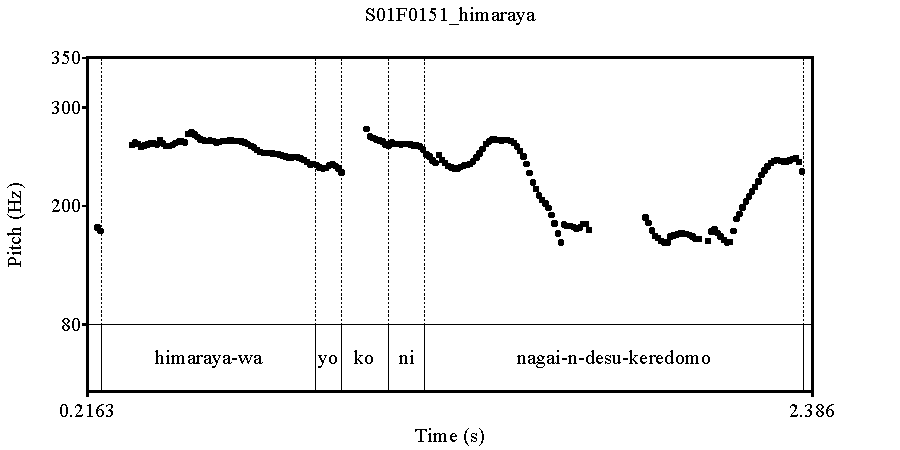
\includegraphics[width=.6\textwidth]{sounds/S01F0151_himaraya.pdf}
	\caption{Pitch contour of c in \ref{S01F0151_himaraya}c}
	\label{S01F0151_himarayaF}
	\end{center}
%\end{minipage}
\end{figure}
\begin{figure}
%\begin{minipage}{0.5\textwidth}
	\begin{center}
	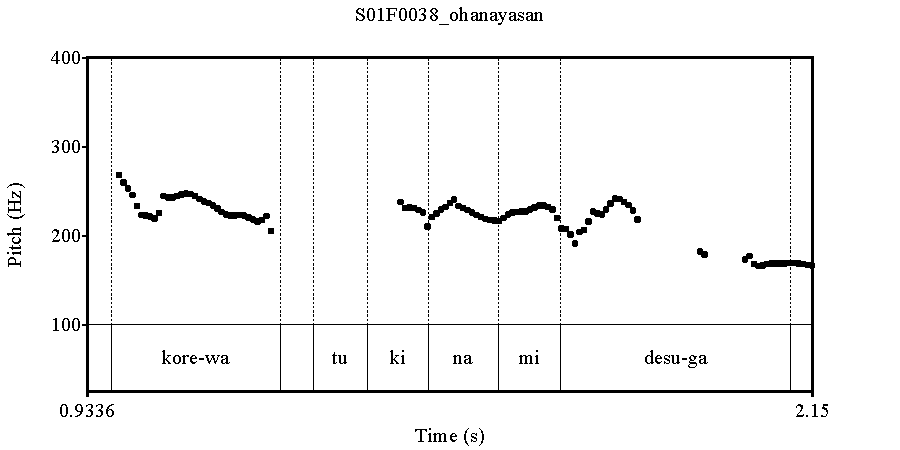
\includegraphics[width=.6\textwidth]{sounds/S01F0038_ohanayasan.pdf}
	\caption{Pitch contour of a in \ref{S01F0038_ohanayasan}a}
	\label{S01F0038_ohanayasanF}
	\end{center}
%\end{minipage}
\end{figure}
\begin{figure}
%\begin{minipage}{0.5\textwidth}
	\begin{center}
	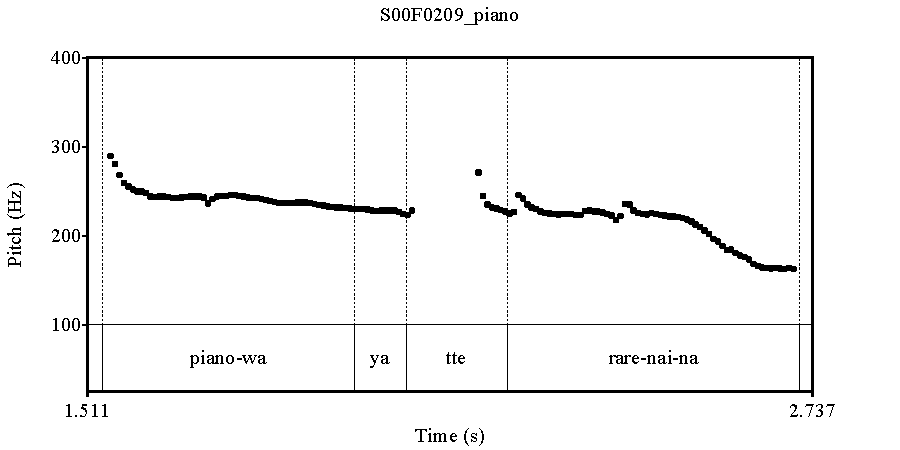
\includegraphics[width=.6\textwidth]{sounds/S00F0209_piano.pdf}
	\caption{Pitch contour of \ref{S00F0209_piano}}
	\label{S00F0209_pianoF}
	\end{center}
%\end{minipage}
\end{figure}


Also,
when the clause is in a special status and is uttered faster,
elements coded by \isi{topic} markers are typically uttered in \isi{clausal} IUs.
For example, inserted clauses are uttered faster relative to other utterances and their \isi{pitch} is lower than the surrounding utterances.
In \Next, where the speaker explains Everest treks and which course she took,
she inserts the clause describing the geometry of the Himalayas in \Next[c].
This clause contains an element coded by a \isi{topic} marker, i.e., \ci{himaraya-wa} `Himalaya-\ci{wa}',
which is uttered in a \isi{clausal} IU.
%
\ex.\label{S01F0151_himaraya}
 \ag. de watasi-ga \tp{\dvline} zissaini \tp{\dvline} it-ta \tp{\dvline} torekkingu-koosu-wa \tp{\dvline} \\
 	then \ab{1}\ab{sg}-\ci{ga} {} actually {} go-\ab{past} {} trekking-course-\ci{wa} {} \\
 \bg. eberesuto-kaidoo-to yob-areru \tp{\dvline} masani \tp{\dvline} \\
 	Everest-trail-\ab{quot} call-\ab{pass} {} exactly {} \\
 \bg. ee \EM{himaraya-wa} yokoni \EMi{nagai}-n-desu-keredomo \tp{\dvline} \\
 	\ab{fl} Himalaya-\ci{wa} horizontally long-\ab{nmlz}-\ab{cop}.\ab{plt}-though {} \\
 \bg. ee sono \tp{\dvline} ee higasi-gawa-ni ataru \tp{\dvline} \\
 	\ab{fl} that {} \ab{fl} east-side-\ab{dat} correspond {} \\
 \bg. eberesuto-o \tp{\dvline} nn -ni  mukat-te iku \tp{\dvline} ruuto-desu \\
 	Everest-\ci{o} {} \ab{fl} -\ab{dat} face-and go {} route-\ab{cop}.\ab{plt} \\
	`The course I took for trekking is called the Everest Trail, which exactly, \EM{uh the Himalayas are long horisontally}, uh on the east side is Everest and we walked toward Everest.'
	\src{S01F0151: 89.71-105.25}
%S01F0151|00089708L|89.708387|105.254992|L|で私が実際に(0.207)行った(0.691)トレッキングコースはエベレスト街道と呼ばれる(0.439)まさに(0.136)(F えー)ヒマラヤは横に長いんですけれども(0.356)(F えー)その(0.219)(F えー)東側に当たるエベレスト(D2 を)(1.065)(F んー)に向かって行く(0.174)ルートです|[文末]|

As shown in Figure \ref{S01F0151_himarayaF},
the F$_{0}$ peak of \ci{himaraya-wa} `Himalaya-\ci{wa}' is higher than
that of the following predicate;
therefore there is no IU boundary between the noun and the predicate.%
	\footnote{
	In \ref{S01F0151_himaraya}, \isi{pitch range} difference cannot be used
	to determine the IU boundary
	because the F$_{0}$ of the phrase \ci{himaraya-wa} is always high
	and hence one cannot meaningfully measure the \isi{pitch range}.
	In this case, the IU boundary is identified after the phrase in question
	if the F$_{0}$ peak of the phrase is lower than that of the following phrase.
	In \ref{S01F0151_himaraya}, the F$_{0}$ peak of \ci{himaraya-wa} is higher than that of the predicate.
	Therefore, the IU boundary is not identified after the phrase \ci{himaraya-wa}
	\cite[see][p.~420 ff.]{igarashietal06}.
	}
In a similar way,
in \Next, where the speaker talks about her childhood dream,
she comments on her dream in the inserted clause \Next[a].
%
\ex.\label{S01F0038_ohanayasan}
 \ag. maa \EM{kore-wa} \EMi{tukinami}-desu-ga \tp{\dvline} \\
 		\ab{fl} this-\ci{wa} ordinary-\ab{cop}.\ab{plt}-though {} \\
		`This (dream) might be too ordinary, but'
 \b. because I liked beautiful flowers,
 \b. (my dream was) florist.
  \src{S01F0038: 53.90-58.93}
%S01F0038|00053900L|53.899807|58.929682|L|(F まー)これは月並みですが(F あの)お花が凄い奇麗で好きだからということで(0.322)(F えー)お花屋さん||体言止

Figure \ref{S01F0038_ohanayasanF} shows the \isi{pitch contour} of \Last[a].
As in the figure,
the F$_{0}$ peak of the \isi{topic} phrase \ci{kore-wa} `this-\ci{wa}' is higher than that of the predicate.
Therefore, there is no IU boundary after \ci{kore-wa}.

Another type of topic-coded element uttered in an \isi{clausal} IU is
embedded in a noun-modifier clause or quotation clause.
For example, in \Next[a],
\ci{piano-wa} `piano-\ci{wa}' is embedded in a quotation clause;
the clause is the content of what the speaker thought.
%
\ex.\label{S00F0209_piano}
 \ag. aa moo \tp{\dvline} kore-wa totemo \EM{piano-wa} \EMi{yat}-te-rare-nai-na-to \ul{\ul{omot}}-tara \tp{\dvline} \\
 	oh any.more {} this-\ci{wa} ever piano-\ci{wa} do-\ab{prog}-\ab{cap}-\ab{neg}-\ab{fp}-\ab{quot} think-\ab{cond} {} \\
	`When I thought that (I) cannot play \isi{piano} any more,'
 \b. it was so painful that I could not stand.
  \src{S00F0209: 214.53-219.84}
%S00F0209|00214526L|214.526341|219.842418|L|(F あー)もうこれはとてもピアノはやってられないなと思ったらもう苦しくて苦しくて仕方(D な)(0.112)がなくて|/テ節/|

As indicated in Figure \ref{S00F0209_pianoF},
which shows the \isi{pitch contour} of \Last[a],
the F$_{0}$ peak of the \isi{topic} phrase \ci{piano-wa} is higher than that of the predicate and the whole clause is interpreted as a single IU.


%%%----------------------------------------------------
%\subsubsection{Motivations for IUs with topics}\label{MotivationsForTopicPIU}



%%----------------------------------------------------
\subsection{Foci tend to be uttered in clausal IUs}\label{Int:IUISUnitCorp:Focus}

%S and P contribute to forming \isi{clausal} IUs.
%Figure \ref{IUASPF} shows the distribution of phrasal vs.\ \isi{clausal} IUs depending on grammatical function.
%Although it is hard to see from the figure,
%S and P tend to be uttered in \isi{clausal} IUs
%when controlling other features such as the existence of \isi{topic} markers and \isi{word order}.

%%----------------------------------------------------
\subsubsection{\textit{Ga}-coded S and \textit{o}-coded P that appear in clausal IUs}

\begin{table}
 \centering
 \tblcaption{Intonation unit vs.~particles}
 \label{IUParT2}
\begin{tabular}{lrrrrrr}
 \toprule
            & \ci{toiuno-wa} & \ci{wa}       & \ci{mo}       & \ci{ga}       & \ci{o}        & \ci{ni} \\
 \midrule
 Phrasal IU &  64            & 157           &  81           &   270         &  160          & 259  \\
            & \rt{(95.5\%)} & \rt{(83.5\%)}  & \rt{(68.6\%)} & \rt{(60.0\%)} & \rt{(47.1\%)} & \rt{(58.6\%)} \\
 Clausal IU &  3             & 31            &  37           & 180           &  180           & 183  \\ 
            & \rt{(4.5\%)}   & \rt{(16.5\%)} & \rt{(31.4\%)} & \rt{(40.0\%)} & \rt{(52.9\%)} & \rt{(41.4\%)} \\
 \midrule
 Sum        &  67            &  188          &  118          &   450         &  340          &  442 \\
            & \rt{(100\%)}   & \rt{(100\%)} & \rt{(100\%)}   & \rt{(100\%)}  & \rt{(100\%)} & \rt{(100\%)} \\
 \bottomrule
\end{tabular}
\end{table}

\begin{figure}
	\begin{center}
	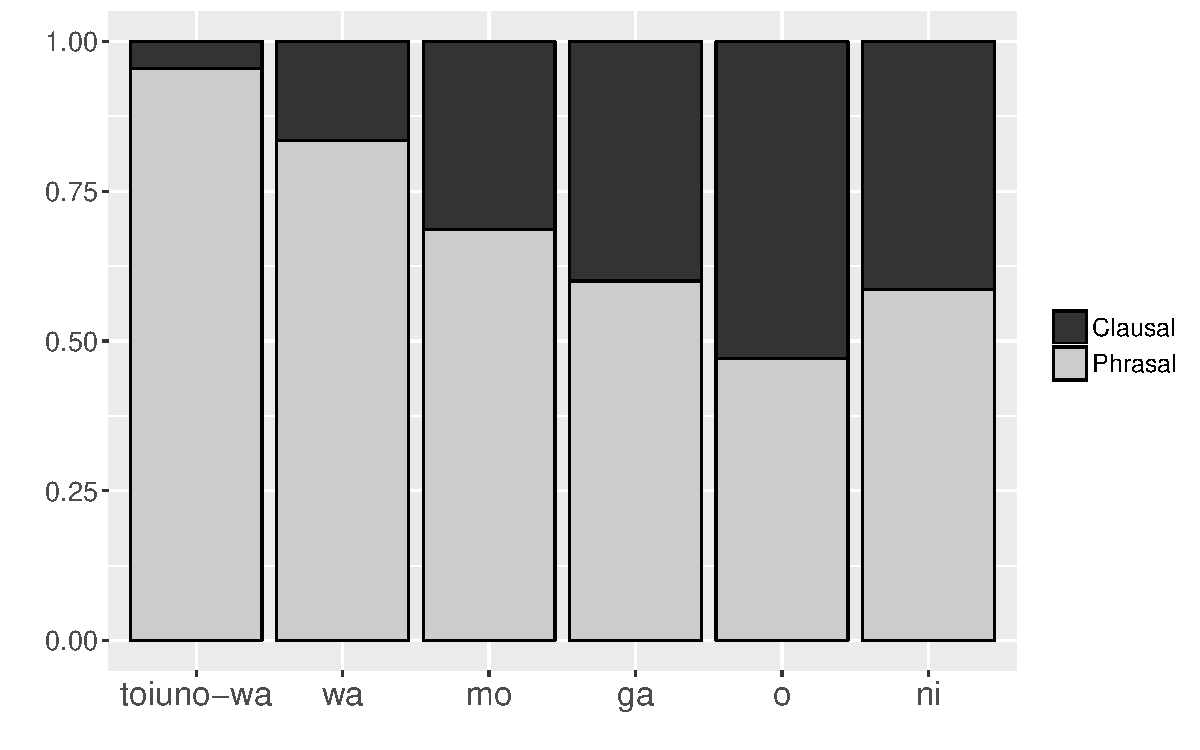
\includegraphics[width=.7\textwidth]{figure/IUPar.pdf}
	\caption{Intonation unit vs.~particles}
	\label{IUParF2}
	\end{center}
\end{figure}

\begin{table}
 \centering
%\begin{minipage}{0.6\textwidth}
 \tblcaption{Intonation unit vs.~grammatical function}
 \label{IUASPT}
\begin{tabular}{lrrrrr}
 \toprule
            & Ex   & A   & S    & P   & Dative \\
 \midrule
 Phrasal IU &  38  & 41  & 463  & 202 & 328  \\
             & \rt{(97.4\%)} & \rt{(80.4\%)} & \rt{(66.0\%)} & \rt{(49.1\%)} & \rt{(62.2\%)} \\
 Clausal IU &   1  & 10  & 239  & 209 & 199  \\ 
             & \rt{(2.6\%)} & \rt{(19.6\%)} & \rt{(34.0\%)} & \rt{(50.9\%)} & \rt{(37.8\%)} \\
 \midrule
 Sum        &  39  & 51   & 702 & 411 & 527 \\
             & \rt{(100\%)} & \rt{(100\%)} & \rt{(100\%)} & \rt{(100\%)} & \rt{(100\%)} \\
 \bottomrule
\end{tabular}
%      Phrasal Clausal
%  Ex       38       1
%  A        41      10
%  S       463     239
%  P       202     209
%  DAT     328     199
%\end{minipage}
\end{table}

\begin{figure}
%\begin{minipage}{0.5\textwidth}
	\begin{center}
	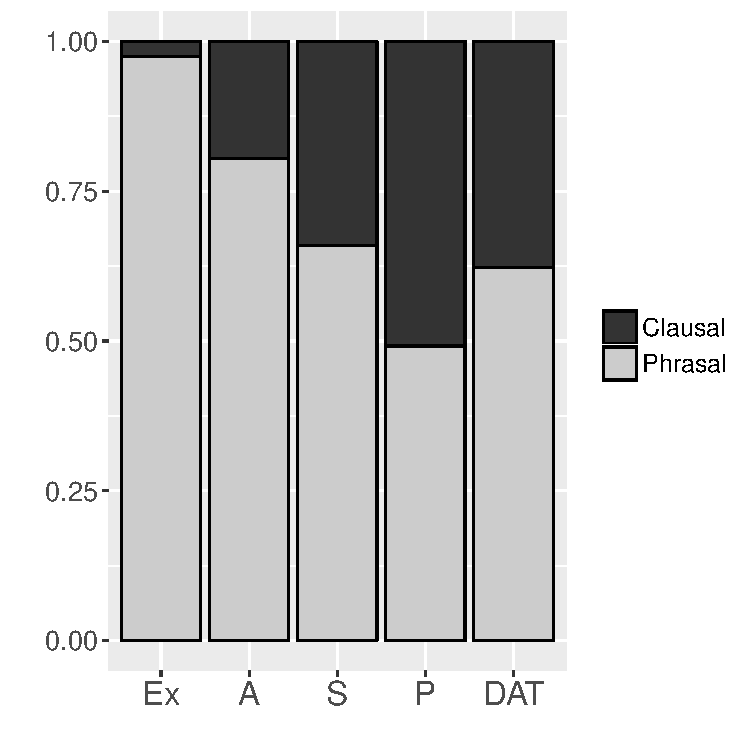
\includegraphics[width=.5\textwidth]{figure/IUASP.pdf}
	\caption{Intonation unit vs.~grammatical function}
	\label{IUASPF}
	\end{center}
%\end{minipage}
\end{figure}

Table \ref{IUParT} and Figure \ref{IUParF},
repeated here as Table \ref{IUParT2} and Figure \ref{IUParF2},
indicates that \ci{ga}- and \ci{o}-coded elements are more likely to
appear in \isi{clausal} IUs than those coded by \isi{topic} markers.
In terms of grammatical function,
it turned out that especially Ss are more likely to be uttered in
\isi{clausal} IUs than As,
as shown in Table \ref{IUASPT} and Figure \ref{IUASPF},
which show the distribution of grammatical function in terms of \isi{intonation unit} regardless of whether elements are coded by \isi{topic} markers or case markers.
Since \ci{ga} and \ci{o} codes focus and
S and P also correlate with focus,
it is reasonable to conclude that
focus in general tends to appear in \isi{clausal} IUs.

\Next[b] is an example of S in \isi{clausal} IUs.
The element \ci{o-hanasi-ga} `\ab{plt}-speech-\ci{ga}'
is uttered in a \isi{clausal} IU.
%
\ex.\label{S00M0221_ohanashi}
 \a. our way of collecting debt might be problematic,
 \bg. oo mina-san \tp{\dvline} zisyuku suru-yooni-to iu \tp{\dvline} \EM{o-hanasi-ga} \EMi{de}-masi-te \tp{\dvline} \\
 	\ab{fl} everyone-\ab{hon} {} control do-\ab{imp}-\ab{quot} say {} \ab{plt}-speech-\ci{ga} come.out-\ab{plt}-and {} \\
 		`somebody proposed that employees should improve the method.'
	\src{S00M0221: 503.23-511.02}
%S00M0221|00503228L|503.227748|511.024933|L|我が社の(0.454)回収方法も少し問題があるんではないかと(1.099)(F おー)皆さん自粛するようにという(0.172)お話が出まして|/テ節/|

As shown in Figure \ref{S00M0221_ohanashiF},
there is no \isi{pitch reset} in the \isi{first mora} of the predicate.
Also,
the \isi{pitch range} of \ci{o-hanasi-ga} `\ab{plt}-speech-\ci{ga}' is larger
than that of the predicate \ci{de-masi-te} `come.out-\ab{plt}-and',
which indicates that the S element and the predicate are uttered in a single IU.

In a similar vein, in \Next,
whose \isi{pitch contour} is shown in Figure \ref{S05M1236_shikitariF},
the S element \ci{sikitari-ga} `tradition-\ci{ga}' and the predicate
are uttered in a single IU;
there is no \isi{pitch reset} observed in the \isi{first mora} of the predicate.
%
\exg.\label{S05M1236_shikitari}hizyooni kanasii \tp{\dvline} anoo \tp{\dvline} \EM{sikitari-ga} \EMi{ari}-masi-te \tp{\dvline} \\
	very sad {} \ab{fl} {} tradition-\ci{ga} exist-\ab{plt}-and {} \\
	`There was a very sad tradition...'
	 \src{S05M1236: 297.99-305.33}
%S05M1236|00297989L|297.989052|305.326268|L|でその人はこう(0.176)毎日消防服を着てるというですね(0.679)非常に悲しい(0.544)(F あのー)(0.284)しきたりがありまして|/テ節/|

\Next[a] is an example of P uttered in a \isi{clausal} IU.
%
\ex.\label{S01M0182_license}
 \ag. ee zyaa \tp{\dvline} ano \EM{puro-raisensu-o} \EMi{tori}-tai-toka \tp{\dvline} \\
 		\ab{fl} then {} \ab{fl} professional-license-\ci{o} take-want-\ab{hdg} {} \\
		`OK, next, (I) wanna take a professional (boxing) license, or something like that,'
 \b. (I) started to think like this.
  \src{S01M0182: 251.43-257.40}
%S01M0182|00251426L|251.425956|257.399081|L|(F えー)じゃ(F あの)プロライセンスを取りたいとか(1.008)ええ(0.104)そういったことに走りまして|/テ節/|

As shown in Figure \ref{S01M0182_licenseF},
since there is no \isi{pitch reset} at the \isi{first mora} of the predicate \ci{tori-tai} `take-want' and the \isi{pitch range} of the element \ci{puro-raisensu-o} `professional-license-\ci{o}' is larger than that of the predicate,
there is no IU boundary after the element \ci{puro-raisensu-o} `professional-license-\ci{o}'.

Similarly, in \Next[c],
whose \isi{pitch contour} is shown in Figure \ref{S02F0100_shujutsuF},
the clause is uttered in a single IU.
The \isi{pitch range} of the element \ci{syuzyutu-o} `operation-\ci{o}'
is larger than that of the predicate.
%
\ex.\label{S02F0100_shujutsu}
 \a. Since I was young,
 \b. many times (I) stayed in the hospital and
 \bg. \EM{syuzyutu-o} \EMi{uke}-tei-tari \tp{\dvline} si-tei-ta-node \tp{\dvline} \\
 		operation-\ci{o} receive-\ab{prog}-\ab{hdg} {} do-\ab{prog}-\ab{past}-because {} \\
		`received operations, so'
 \b. when I die,
 \b. (I) was thinking that (I) would probably die in an accident or from disease.
  \src{S02F0100: 387.22-399.08}
%S02F0100|00387218L|387.218022|399.075|L|で(0.285)あたしは今までに小さい頃から何回も入院したり手術を受けていたり(0.628)していたので私が(0.276)もしも死ぬ時は(0.272)事故や寿命でなく病気だと(0.362)漠然と思っていました|[文末]|

\begin{figure}
%\begin{minipage}{0.5\textwidth}
	\begin{center}
	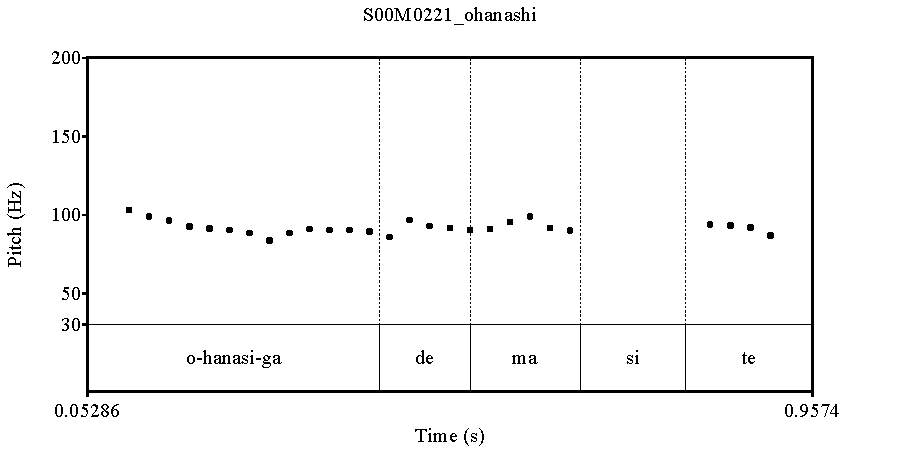
\includegraphics[width=.6\textwidth]{sounds/S00M0221_ohanashi.pdf}
	\caption{Pitch contour of \ref{S00M0221_ohanashi}}
	\label{S00M0221_ohanashiF}
	\end{center}
%\end{minipage}
\end{figure}
\begin{figure}
%\begin{minipage}{0.5\textwidth}
	\begin{center}
	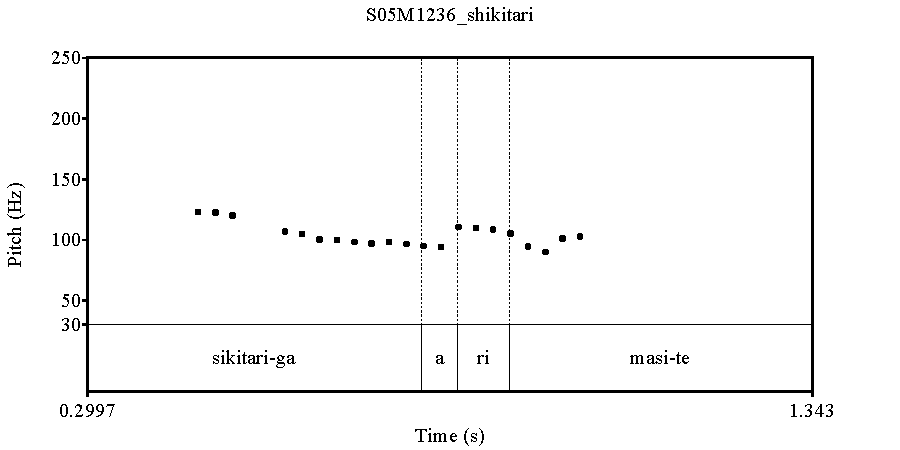
\includegraphics[width=.6\textwidth]{sounds/S05M1236_shikitari.pdf}
	\caption{Pitch contour of \ref{S05M1236_shikitari}}
	\label{S05M1236_shikitariF}
	\end{center}
%\end{minipage}
\end{figure}
\begin{figure}
%\begin{minipage}{0.5\textwidth}
	\begin{center}
	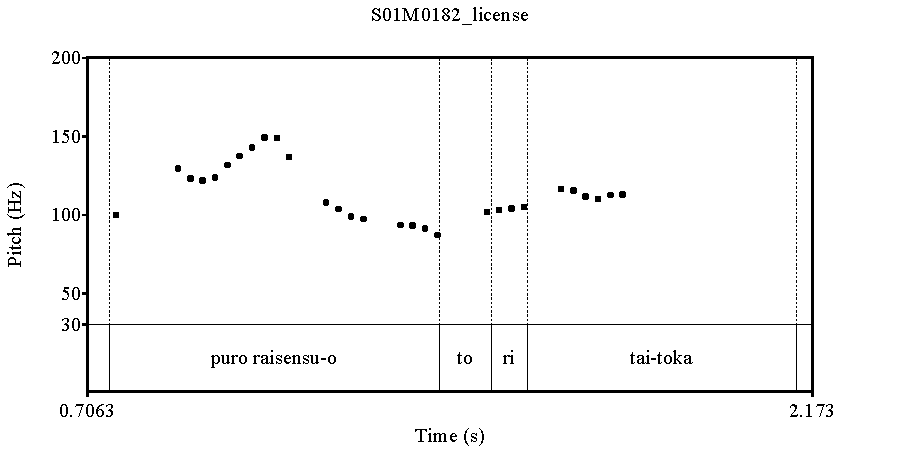
\includegraphics[width=.6\textwidth]{sounds/S01M0182_license.pdf}
	\caption{Pitch contour of a in \ref{S01M0182_license}}
	\label{S01M0182_licenseF}
	\end{center}
%\end{minipage}
\end{figure}
\begin{figure}
%\begin{minipage}{0.5\textwidth}
	\begin{center}
	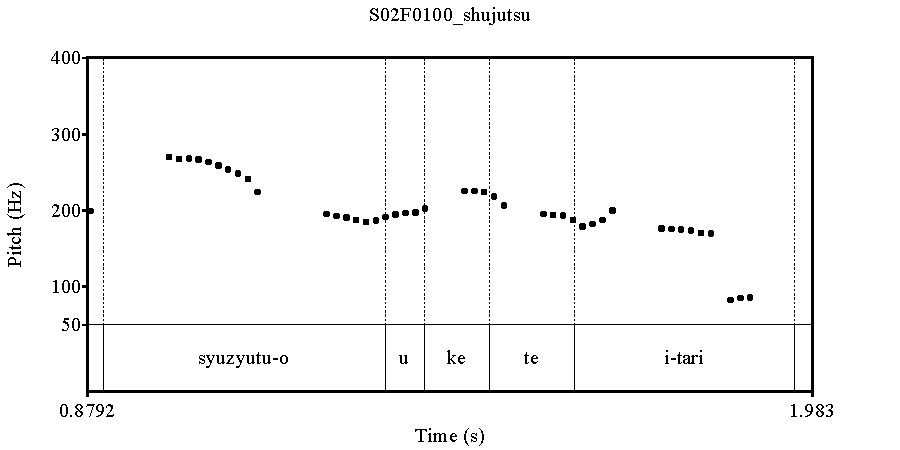
\includegraphics[width=.6\textwidth]{sounds/S02F0100_shujutsu.pdf}
	\caption{Pitch contour of c in \ref{S02F0100_shujutsu}}
	\label{S02F0100_shujutsuF}
	\end{center}
%\end{minipage}
\end{figure}


%%----------------------------------------------------
\subsubsection{\textit{Ga}-coded S and \textit{o}-coded P that appear in phrasal IUs}\label{Int:Cor:Focus:PIU}


\begin{figure}
%\begin{minipage}{0.5\textwidth}
	\begin{center}
	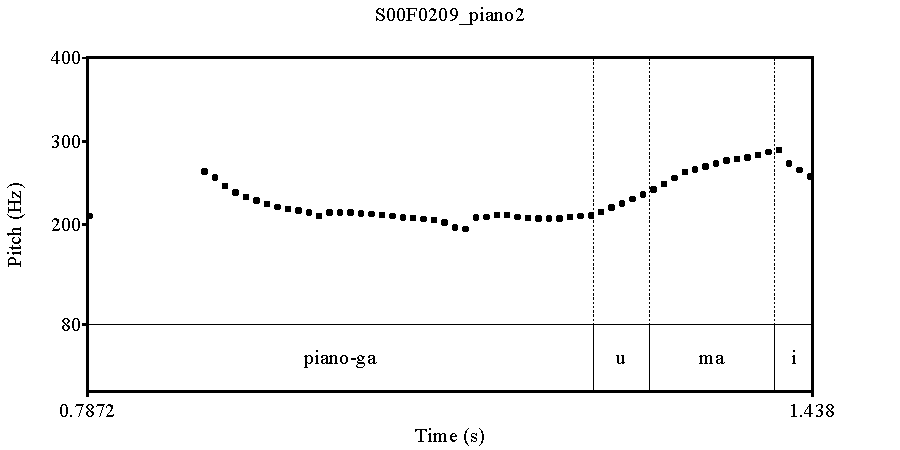
\includegraphics[width=.5\textwidth]{sounds/S00F0209_piano2.pdf}
	\caption{Pitch contour of a in \ref{S00F0209_piano2}}
	\label{S00F0209_piano2F}
	\end{center}
%\end{minipage}
\end{figure}
\begin{figure}
%\begin{minipage}{0.5\textwidth}
	\begin{center}
	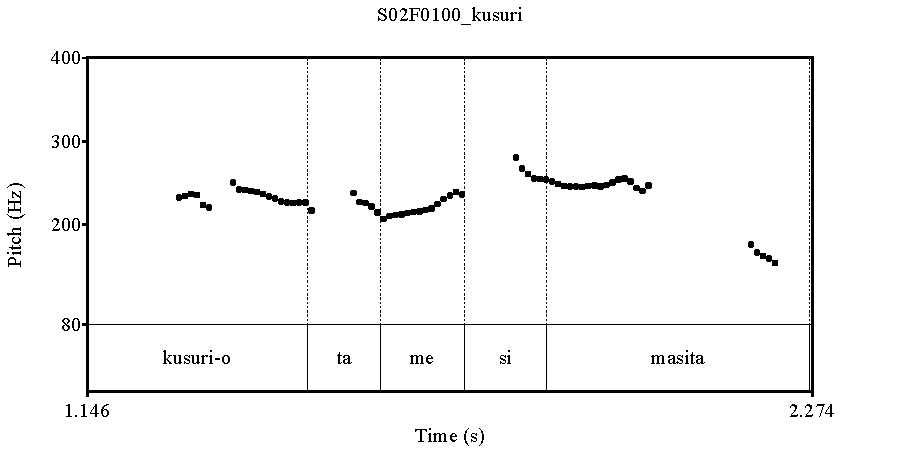
\includegraphics[width=.6\textwidth]{sounds/S02F0100_kusuri_piu.pdf}
	\caption{Pitch contour of a in \ref{S02F0100_kusuri}}
	\label{S02F0100_kusuri_piuF}
	\end{center}
%\end{minipage}
\end{figure}
\begin{figure}
%\begin{minipage}{0.5\textwidth}
	\begin{center}
	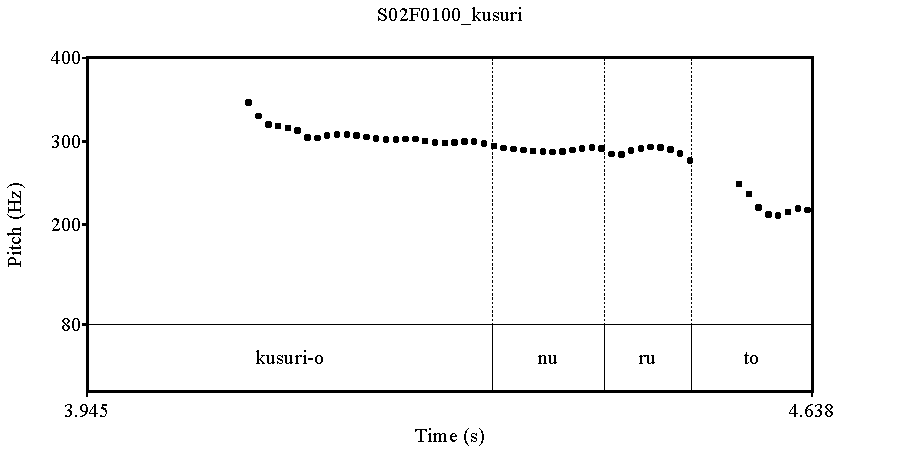
\includegraphics[width=.6\textwidth]{sounds/S02F0100_kusuri_ciu.pdf}
	\caption{Pitch contour of b in \ref{S02F0100_kusuri}}
	\label{S02F0100_kusuri_ciuF}
	\end{center}
%\end{minipage}
\end{figure}

Here, I discuss \ci{ga}-coded S and \ci{o}-coded P that
appear in phrasal IUs.
Although they are more likely to be uttered in \isi{clausal} IUs than 
those coded by \isi{topic} markers,
there are many of those uttered in phrasal IUs
as shown in Table \ref{IUASPT} and Figure \ref{IUASPF}.
I point out two types of focal elements uttered in phrasal IUs.

The first type of this kind is strongly evoked elements
which are uttered in lower \isi{pitch} than their predicate and
therefore have an IU boundary after these elements.
They are uttered in phrasal IUs for the same reason as pronouns as discussed in \S \ref{Int:Cor:Topic:CIU}.
For example, in \Next, whose \isi{pitch contour} is shown in Figure \ref{S00F0209_piano2F},
\ci{piano} is strongly evoked and is uttered in lower \isi{pitch} than its predicate.
Therefore, the F$_{0}$ range of \ci{piano} is smaller than that of the following predicate and there is an IU boundary between the element \ci{piano} and the predicate.
\ci{Piano} is considered to be strongly evoked
because the speaker mentions it repeatedly throughout her talk.
%
\ex.\label{S00F0209_piano2}
 \ag. zibun-yori \EM{piano-ga} \tp{\dvline} \EMi{umai} hito-ga yononaka-ni-wa takusan \tp{\dvline} \\
          self-than piano-\ci{ga} {} good.at person-\ci{ga} world-\ab{dat}-\ci{wa} a.lot {} \\
 \bg. takusan iru... \\
      many exist... \\
      `There are so many people who are better at (playing) \isi{piano} than me...'
 \b.[] \src{S00F0209: 204.28-206.81}

Similarly, in \Next[a], whose \isi{pitch contour} is shown in Figure \ref{S02F0100_kusuri_piuF},
\ci{kusuri} `medicine' is strongly evoked and uttered in lower \isi{pitch} than the predicate \ci{tamesu} `try'.
\ci{Kusuri} `medicine' is strongly evoked because
it also has been mentioned immediately before \Next[a],
as indicated by \ci{sono} `that'.
%
\ex.\label{S02F0100_kusuri}
 \ag. sono s \EM{kusuri-o} \tp{\dvline} \EMi{tamesi}-masi-ta \tp{\dvline} \\
       that \ab{frg} medicine-\ci{o} {} try-\ab{plt}-\ab{past} {} \\
       `(I) tried that medicine (because I was told that there was no other way).'
  \bg. de \tp{\dvline} tasikani sono \EM{kusuri-o} nuru-to \tp{\dvline} \\
       then {} certainly that medicine-\ci{o} put-\ab{cond} {} \\
       `As the doctor said, when (I) put on the medicine,'
  \b. (my disease) becomes a little bit better...
  \src{S02F0100: 155.34-159.32}
%S02F0100|00155336L|155.335655|159.319497|L|これより他に方法がないと言われてその(D す)薬を試しました|[文末]|
%S02F0100|00159770L|159.770013|163.130548|L|で(0.375)確かにその薬を塗ると少し良くなるんですが|/並列節ガ/|

However, in \Last[b], which immediately follows \Last[a],
the F$_{0}$ peak of \ci{kusuri} `medicine' is higher than that of the predicate \ci{nuru} `put on',
as shown in Figure \ref{S02F0100_kusuri_ciuF}.
This contrasts with what I have claimed so far.
I believe that the F$_{0}$ peak of \ci{kusuri} in \Last[b] is higher than that of the predicate because this appears sentence-initially.
Japanese is a clause-chaining language,
which combines multiple clauses to form a thematic unit \cite{longacre85,martin92,givon01}.
F$_{0}$ of sentence-initial clauses are the highest and it declines as the sentence goes on \cite{koisoishimoto12,ishimotokoiso12,ishimotokoiso13}.
Therefore,
the elements in the sentence-initial position are the highest among other elements.
As I have argued in \S \ref{Int:Cor:Topic:CIU},
a pair of strongly evoked element and the following phrase should be considered to form a single processing unit.
As in Figure \ref{S00F0209_piano2F} - \ref{S02F0100_kusuri_ciuF},
there is no pause or \isi{vowel} lengthening between the \isi{anaphoric element} and the predicate,
which typically appear IU-finally.
This supports the notion that they should be integrated into a single unit at the level higher than \isi{intonation unit}.


The second type is not as clear as the first one.
I am not sure whether examples of the second type share the same characteristics.
Rather, it is likely that they are still heterogeneous.
Here I try to capture some characteristics they have.
In some examples of the second type,
the element is non-\isi{anaphoric} and the F$_{0}$ is high,
however, the F$_{0}$ of the predicate is also high for some reason.
Examples of this kind are shown in \Next and \NNext.
In \Next, \ci{kusa} `grass' is non-\isi{anaphoric} and is uttered with prominence,
but there is a \isi{pitch reset} before the predicate, which has its own F$_{0}$ peak as in Figure \ref{S00F0014_kusaF}.
%
\ex.\label{S00F0014_kusa}
 \ag. \EM{kusa-ga} \tp{\dvline} \EMi{hae}-te ki-ta \tp{\dvline} tokoro-ni \tp{\dvline} \\
 		grass-\ci{ga} {} grow-and come-\ab{past} {} place-\ab{dat} {} \\
		`The place where grasses grow up'
 \b. some people build houses...
  \src{S00F0014: 276.80-279.30}
%S00F0014|00271393L|271.392628|283.29407|L|(F あの)本当に(F ん)何て言うんでしょう溶岩の中に(0.369)みんなが<FV>それぞれ(F あの)勝手に草が生えてきたところに(0.36)家を建てたり(0.267)色々な生活の場を(0.28)築いてった(0.118)ようなところでした|[文末]|

In \Next,
in a similar vein,
there is a \isi{pitch reset} before the predicate;
the \isi{non-anaphoric element} \ci{tatoe} `metaphor' and the predicate \ci{warui} `bad' have their own F$_{0}$ peak as in Figure \ref{S00M0199_tatoeF}.
%
\ex.\label{S00M0199_tatoe}
 \ag. ee tyotto \tp{\dvline} \EM{tatoe-ga} \tp{\dvline} \EMi{warui}-n-desu-ga \tp{\dvline} \\
 		\ab{fl} a.bit {} metaphor-\ci{ga} {} bad-\ab{nmlz}-\ab{cop}.\ab{plt}-though {} \\
		`This might be a bit bad metaphor, but'
 \b. it's kind of kamikaze-like idea.
  \src{S00M0199: 360.76-365.14}
%S00M0199|00351884L|351.883772|377.653608|L|これはもうまさに(0.432)(F えー)歴史的に(0.112)(F えー)(0.263)もう記述されて(0.116)(F えー)もう民族のアイデンティティーの根幹をなすような(0.336)(F ま)まさに日本で言えば(0.457)(F えー)ちょっと例えが悪いんですが(0.151)(F えー)戦中の(F その)神風的な発想で(0.445)(F えー)コソボ平原において(0.121)もう殆どの人が命をなくすんではないかという(0.412)(F え)名誉な(0.125)名誉ある敗北という言い方されてますが(0.391)によって(0.13)このコソボをオスマントルコによって(0.114)(F えー)(F ま)占領される訳なんですが|/並列節ガ/|

\begin{figure}
%\begin{minipage}{0.5\textwidth}
	\begin{center}
	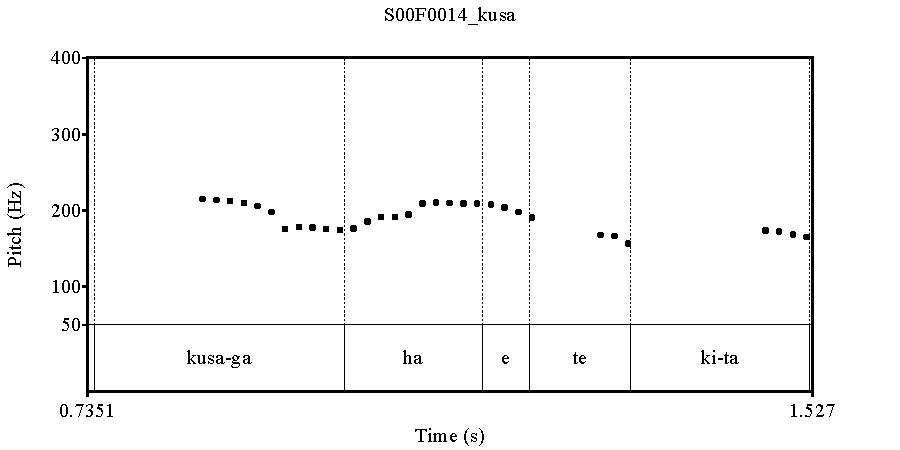
\includegraphics[width=.5\textwidth]{sounds/S00F0014_kusa.pdf}
	\caption{Pitch contour of a in \ref{S00F0014_kusa}}
	\label{S00F0014_kusaF}
	\end{center}
%\end{minipage}
\end{figure}
\begin{figure}
%\begin{minipage}{0.5\textwidth}
	\begin{center}
	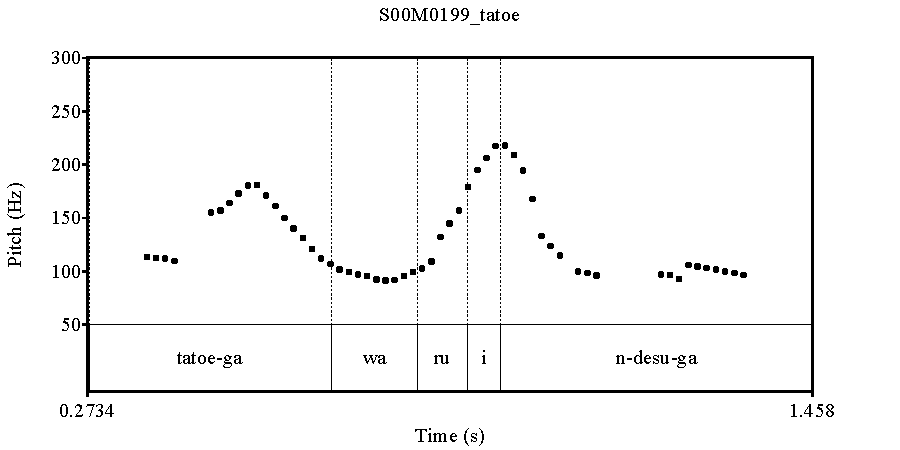
\includegraphics[width=.5\textwidth]{sounds/S00M0199_tatoe.pdf}
	\caption{Pitch contour of a in \ref{S00M0199_tatoe}}
	\label{S00M0199_tatoeF}
	\end{center}
%\end{minipage}
\end{figure}
%
In other examples of the second type,
non-\isi{anaphoric} elements are uttered in \isi{low pitch} without prominence
as though they are strongly evoked.
In example \Next,
the brand-new element \ci{nyuukinbi} `the deadline of repayment' is produced in \isi{low pitch} against our prediction
as shown in Figure \ref{S00M0221_nyuukimbiF}.
%
\ex.\label{S00M0221_nyuukimbi}
 \a. ``Do you forget (about the deadline)?''
 \bg. oo \tp{\dvline} \EM{nyuukinbi-ga} \tp{\dvline} \EMi{sugi}-te ori-masu-toiu koto-de \tp{\dvline} \\
      \ab{fl} {} deadline-\ci{ga} {} pass-and \ab{prog}.\ab{plt}-\ab{plt}-\ab{quot} thing-\ab{cop} \\
      ```The deadline of repayment has passed'' something like that...'
  \b.[] \src{S00M0221: 220.24-225.28}
%S00M0221|00220236L|220.235607|232.473221|L|(F おー)取り敢えずお忘れですかと(1.176)(F おー)入金日が過ぎておりますということで(0.676)(F えー)遅れの浅い人から(0.101)どんどんどんどん(0.157)(F おー)回すという形で(0.121)(F えー)(0.157)仕事の方行なっていました|[文末]|

In this case, however,
\ci{nyuukinbi} `the deadline of repayment' can be also regarded to be \isi{inferable} through the previous context,
because the speaker has been talking about the people who did not return money,
although the speaker has not specifically mentioned \ci{nyuukinbi} `the deadline'.
However, it is more natural for \isi{inferable} elements
to acquire their own \isi{pitch peak}.
%Therefore, in this example,
%the element is similar to strongly active elements and there is no wonder that it is uttered in \isi{low pitch}.
%Since it is similar to a strongly active element,
%I argue that the element and the predicate should form a single processing unit for the same reason I argued in \S \ref{TopCIU}.

Moreover,
there are also cases where perfectly brand-new elements are uttered in \isi{low pitch} as if they were strongly evoked.
In \Next,
neither the element \ci{kyoomi} `interest' nor the related concepts have been mentioned in the previous \isi{discourse},
while it is still uttered in \isi{low pitch} as in Figure \ref{S00F0014_kyoomiF}.
%
\ex.\label{S00F0014_kyoomi}
 \ag. ee sono ritoo-no \tp{\dvline} hoo-ni \EM{kyoomi-o} \tp{\dvline} \EMi{moti} hazime-masi-te \tp{\dvline} \\
      \ab{fl} \ab{fl} neighbour.island-\ab{gen} {} direction-to interest-\ci{o} {} have start-\ab{plt}-and {} \\
      `(We) started to be interested in neighbour islands (in Hawaii),'
 \b. and the first island in Hawaii we went to is Maui.
 \src{S00F0014: 149.92-156.93}
%S00F0014|00149920L|149.919959|153.334445|L|で(0.325)(F えー)(F その)離島の方に(F その)興味を持ち始めまして|/テ節/|
%S00F0014|00153648L|153.648299|156.934498|L|一番最初(F その)ハワイへ(0.296)行ったのはマウイ島だったんですね|[文末]|

I do not have a clear explanation for why this happens.
Intuitively, the F$_{0}$ peak can be either on the element \ci{kyoomi} `interest' or on the predicate \ci{moti} `have'
and the nuance does not change.
However, it is unnatural if both the element and the predicate have their own F$_{0}$ peaks.
Typically there is no pause or \isi{vowel} lengthening between the element and the predicate in this type of example.
Therefore, I tentatively conclude that uttering both the element and the predicate in a coherent \isi{pitch contour} is important and I leave open the question of which one should have the F$_{0}$ peak.
I am inclined to think that the element and the predicate form a single processing unit.

\begin{figure}
%\begin{minipage}{0.5\textwidth}
	\begin{center}
	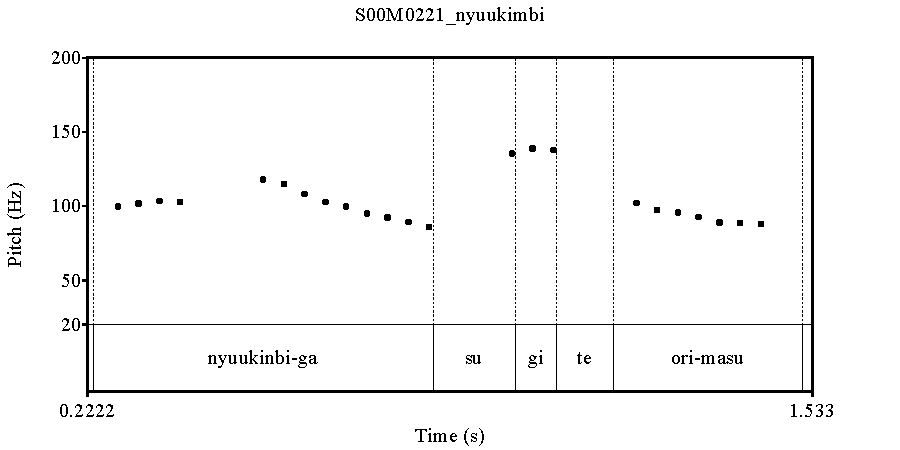
\includegraphics[width=.5\textwidth]{sounds/S00M0221_nyuukimbi.pdf}
	\caption{Pitch contour of b in \ref{S00M0221_nyuukimbi}}
	\label{S00M0221_nyuukimbiF}
	\end{center}
%\end{minipage}
\end{figure}
\begin{figure}
%\begin{minipage}{0.5\textwidth}
	\begin{center}
	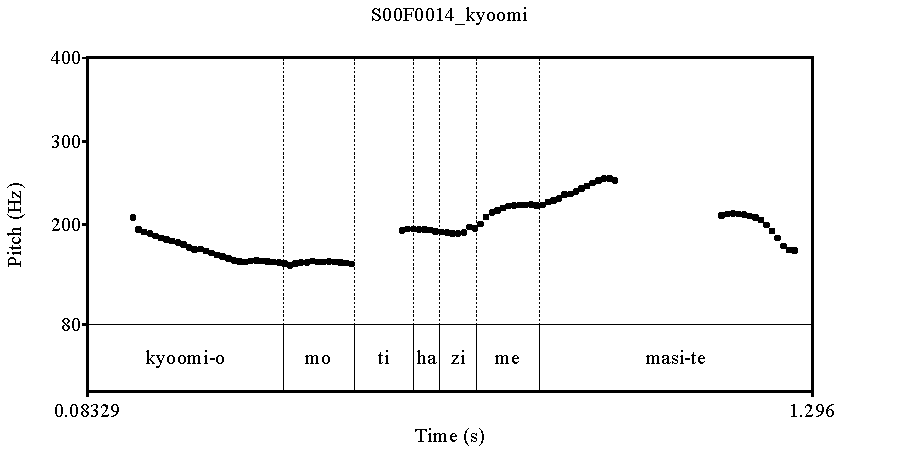
\includegraphics[width=.5\textwidth]{sounds/S00F0014_kyoomi.pdf}
	\caption{Pitch contour of a in \ref{S00F0014_kyoomi}}
	\label{S00F0014_kyoomiF}
	\end{center}
%\end{minipage}
\end{figure}



%%----------------------------------------------------
%\subsubsection{Motivations for S and P appearing in clausal IUs}\label{MotivationsForSPCIU}




%%----------------------------------------------------
%\subsection{Remaining question}



%%% LOCについてもっと議論

%\begin{itemize}
%	\item \EM{Locative} (and temporal) expressions often consist of \EM{phrasal IUs}
%	\item function as a scene setting
%	\item consist of a phrasal IU
%\end{itemize}
%\ex. \ag. \EM{kono} \EM{aida-mo} a ee \EM{kokugikan-de} \tp{\dvline} e nihon-taitoru-matti-ga itutu aru \tp{\dvline} \\
%		this interval-also \ab{fl} \ab{fl} Kokugikan-\ab{loc} \ab{fl} Japan-title-match-\ab{nom} five exist \\
%		`A few days ago also, at Kokugikan, there are five Japan title matches,'
%	\bg. ee taitoru-matti-ga at-ta-n-desu-kedomo \tp{\dvline} \\
%		\ab{fl} title-match-\ab{nom} exist-\ab{past}-\ab{nmlz}-\ab{plt}-though \\
%		`there were title matches...'
%		\hfill{(\code{S01M0182: 630.52-637.04})}
%
%この間もあえー国技館で\tp{\dvline}え日本タイトルマッチが五つある\tp{\dvline}
%えータイトルマッチがあったんですけども\tp{\dvline} (S01M0182: 630.52-637.04)
%\exg. \EM{zissai-ni-wa} \tp{\dvline} ita-no \EM{ue-ni} \tp{\dvline} mattoresu-mitaina-no-ga \tp{\dvline} sii-te-aru-dake-de \tp{\dvline} \\
%	actually-\ci{ni}-\ci{wa} wood-\ab{gen} above-\ab{loc} mattress-like-\ab{nmlz}-\ab{nom} roll-and-exist-only-and \\
%	`Actually, it (the bed) was only a mattress on a piece of wood.'
%		\hfill{(\code{S01M0182: 630.52-637.04})}
%
%実際には\tp{\dvline}板の上に\tp{\dvline}マットレスみたいなのが\tp{\dvline}敷いてあるだけで\tp{\dvline} (S01F0151: 441.33-444.88)


%%----------------------------------------------------
\subsection{Summary of corpus study}

\begin{figure}
\centering
%\begin{minipage}{0.5\textwidth}
	\begin{center}
	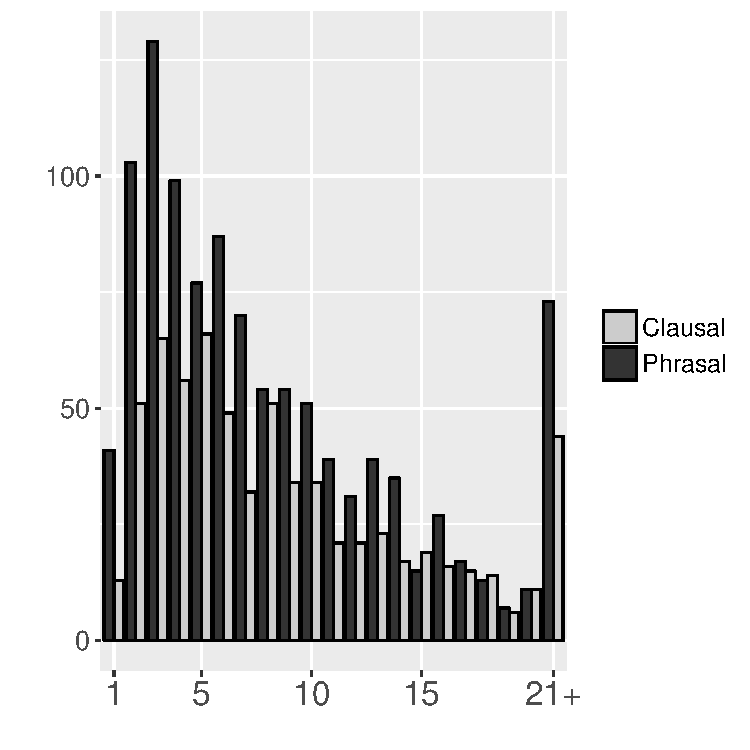
\includegraphics[width=.5\textwidth]{figure/IUWO.pdf}
	\caption{Intonation unit vs.~word order}
	\label{IUWOF}
	\end{center}
%\end{minipage}
\end{figure}



This section argued that
evoked, \isi{inferable}, and declining topics tend to be produced in phrasal IUs,
separately from the IU with the predicate; and
strongly evoked topics are typically produced in \isi{clausal} IUs
together with the IU with the predicate;
whereas foci tend to be produced in \isi{clausal} IUs,
although there are explainable exceptions.

However, as discussed in Chapter \ref{WordOrder},
topics tend to appear clause-initially and foci tend to appear right before the predicate.
An element is more likely to be uttered in \isi{clausal} IUs
if it is closer to the predicate,
which implies that
foci are more likely to be uttered in \isi{clausal} IUs.
Therefore, it is not entirely clear whether \isi{information structure} really
affects the difference between phrasal and \isi{clausal} IUs independent of \isi{word order}.
As an example, let us assume that \Next is a possible \isi{utterance} that the speaker bears in his/her mind.
``(\tp{\dvline})'' indicates a potential IU boundary.
For simplicity,
let us assume that
only one out of the three potential IU boundaries realizes in this \isi{utterance}.
%
\ex. A (\tp{\dvline}$_1$) B (\tp{\dvline}$_2$) C (\tp{\dvline}$_3$) Predicate

If the speaker wants to put an IU boundary in \tp{\dvline}$_1$,
the IU which includes A is a phrasal IU,
whereas the IU which includes B and C is a \isi{clausal} IU
as schematized in \Next.
%
\ex. \fbox{A} \tp{\dvline}$_1$ \fbox{B C Predicate}

On the other hand, if the speaker wants to put the IU boundary in \tp{\dvline}$_2$,
now the IU which includes A and B is a phrasal IU,
whereas the IU which includes C is a \isi{clausal} IU.
This is schematized in \Next.
%
\ex. \fbox{A B} \tp{\dvline}$_2$ \fbox{C Predicate}

This indicate that even though the speaker does not want to put the IU boundary in \tp{\dvline}$_1$,
A are uttered in a phrasal IU because of \tp{\dvline}$_2$ and \tp{\dvline}$_3$;
A is more likely to be uttered in a phrasal IU than B and C because it is uttered earlier.
Similarly, B is more likely to be uttered in a phrasal IU than C.
The effects of \isi{word order} should not be ignored in the distinction between phrasal and \isi{clausal} IUs.
In fact,
as Figure \ref{IUWOF} shows,
earlier elements are more likely to be produced in phrasal IUs
than later elements.

In the next section,
I discuss an experiment, controlling \isi{word order},
and show that topics tend to be followed by an IU boundary,
while foci are not.
%I discuss the relation between \isi{word order} and the phrasal-vs.-\isi{clausal} IU distinction and argue that
%\isi{word order} and IU both reflects human mind processing and one cannot tease them apart.




%%----------------------------------------------------
%%----------------------------------------------------
\section[IU and IS unit: experimental study]{Intonation unit and unit of \isi{information structure}: experimental study}\label{Int:IUISUnitExp}

In the previous sections,
I investigated the corpus of spoken Japanese.
%argued that a unit of \isi{information structure} corresponds to an \isi{intonation unit}.
In this section,
I will show that my argument so far is also supported by a \isi{production experiment} keeping \isi{word order} constant.


%%----------------------------------------------------
\subsection{Method}\label{Int:IUISUnitExp:Meth}

This section gives an overview of the method of the experiment.
First, I explain how stimuli are made (\S \ref{Int:IUISUnitExp:Meth:Sti}),
then go over the procedure of the experiment (\S \ref{Int:IUISUnitExp:Meth:Proc}).
Finally,
I explain how the recordings acquired are annotated (\S \ref{Int:IUISUnitExp:Meth:Anot}).

%%----------------------------------------------------
\subsubsection{Stimuli}\label{Int:IUISUnitExp:Meth:Sti}

First, I made a list of three-mora nouns without accent nucleus (the \isi{pitch} formation is expected to be LHH).
I chose basic words that are used in everyday life,
such as \ci{sakura} `cherry blossom' and \ci{koinu} `puppy'.
I used an electronic dictionary of Japanese called \ci{UniDic}
to search words
\cite{denetal02,denetal07}.%
	\footnote{\url{http://sourceforge.jp/projects/unidic/}}
I chose words of this accent type to
exclude the potential effect of the accent of these words on the following words.
Second, I collected a list of verbs starting with \isi{low pitch}.
The \isi{second mora} of the verbs should be high because the first and the second morae of a word should be distinct as discussed in \S \ref{BackSubSecGeneralChar}.
I chose these words to see the F$_{0}$ difference between the first
and the second morae.
Third, I made 14 pairs of a noun and a \isi{verb} of high collocation using \ci{Case Frame} \cite{kawaharakurohashi06b,kawaharakurohashi06}.%
	\footnote{\url{http://reed.kuee.kyoto-u.ac.jp/cf-search/}}
7 pairs are subject-\isi{verb}, and
the remaining 7 pairs are object-\isi{verb},
using the same noun.
%The nouns can be either subject or object of the verbs.
The stimuli can be schematized as in \Next,
where N indicates noun and V indicates \isi{verb}.
%
\ex. [LHH]$_{N}$ [LH...]$_{V}$

Finally, I made two contexts for each pair;
in one context, the noun is interpreted as \isi{topic},
and in the other context, the noun and the \isi{verb} as a whole are interpreted as focus.

Examples of two kinds of contexts and noun-\isi{verb} pairs are shown in \Next and \NNext.
The target sentence is \ci{koinu yuzut-ta} `(I/we) gave (a/the) puppy'.
In \Next, where the noun is intended to be interpreted as \isi{topic} and the \isi{verb} to be focus,
the referent of the noun \ci{koinu} `puppy' has already been shared between the speaker and the \isi{hearer}.
Only the \isi{verb} \ci{yuzu-ta} `gave' is news to the \isi{hearer}.
In all examples,
the context forces the speakers to assume topics to be unused.
%
\ex.\label{koinut}
\tl{Predicate-focus context}: Yesterday the speaker and his/her friend found an abandoned puppy on the street. The speaker brought it to his/her home. Today, the speaker tells the friend what happened to the puppy.
\ag.[] sooieba [\EM{koinu}]$_{T}$ [\EM{yuzut-ta}]$_{F}$-yo \\
by.the.way puppy give-\ab{past}-\ab{fp} \\
`By the way, (I) gave the puppy (to somebody).'
%	\hfill{\movie{play}{koinut.wav}}

In \Next, on the other hand,
where both the noun and the \isi{verb} are intended to be interpreted as focus,
the referent of the noun \ci{koinu} `puppy' has not been shared.
Not only the \isi{verb} `gave', but also `a puppy' is brand-new to the \isi{hearer}.
%
\ex.\label{koinuf}
 \tl{All-focus context}: The speaker and his/her friend are working in an animal shelter. The friend was absent yesterday and wants to know what happened yesterday.
\ag.[] kinoo-wa [\EM{koinu} \EM{yuzut-ta}]$_{F}$-yo \\
yesterday-\ci{wa} puppy give-\ab{past}-\ab{fp} \\
`Yesterday (we) gave puppies.'
%	\hfill{\movie{play}{koinuf.wav}}


%I collected only nouns without accent nucleus
%because, if a noun has an accent nucleus,
%the \isi{pitch} pattern of the following words might be influenced.
%For example,

After I made stimuli,
I randomized the order of them so that
the same target sentences (with predicate-focus and all-focus contexts)
do not appear adjacent with each other.

%%----------------------------------------------------
\subsubsection{Experimental procedure}\label{Int:IUISUnitExp:Meth:Proc}

I asked seven native speakers of standard Japanese
to read aloud the stimuli.
All of the participants grew up in Tokyo or near Tokyo (such as Saitama), where standard Japanese is spoken.
All of them have lived for more than a year outside of the areas where standard Japanese is not spoken.
Four of the participants are male, and three are female.
I recorded their production using EDIROL (R09-HR) and the internal microphone.

%%----------------------------------------------------
\subsubsection{Coding process}\label{Int:IUISUnitExp:Meth:Anot}

After the recording, I coded their speech using Praat.%
\footnote{\url{http://www.fon.hum.uva.nl/praat/}}
First, I divided each target sentence into morae,
then I divided each mora into a consonant (if any) and a \isi{vowel}.
Second, I measured F$_{0}$ of the midpoint of the vowels with a Praat script.


%%----------------------------------------------------
\subsection{Results}

Figure \ref{Int:fig:Sp1}-\ref{Int:fig:Sp4} show
the F$_{0}$ of vowels of each target sentence based on \isi{information structure}.
The graphs of Speaker 5--7 are omitted.
In the x-axis, \code{n1} indicates the \isi{first mora} of the noun, \code{n2} indicates the \isi{second mora}, and
\code{v1} indicates the \isi{first mora} of the \isi{verb}, and so on.

In some cases, there are less than 14 data points.
This is because some vowels are devoiced.
In standard Japanese, high vowels are often devoiced between two voiceless consonants such as \ci{kusuri} [\tp{k\r*WsWRi}] `medicine'.
However, this is not always the case.
Therefore, the numbers of data points vary depending on the speaker.

The red lines indicate the plot of the \isi{predicate-focus context},
while the blue lines indicate the plot of the all-focus context.
The error bars indicate the standard variations of F$_{0}$.
Although the error bars are too large,
it is clear that there is a \isi{pitch reset} in \code{v1}, i.e., the \isi{first mora} of the \isi{verb},
and the \isi{pitch} rises again in \code{v2}, i.e., the \isi{second mora} of the \isi{verb}.

\begin{figure}
%\begin{minipage}{0.5\textwidth}
	\begin{center}
	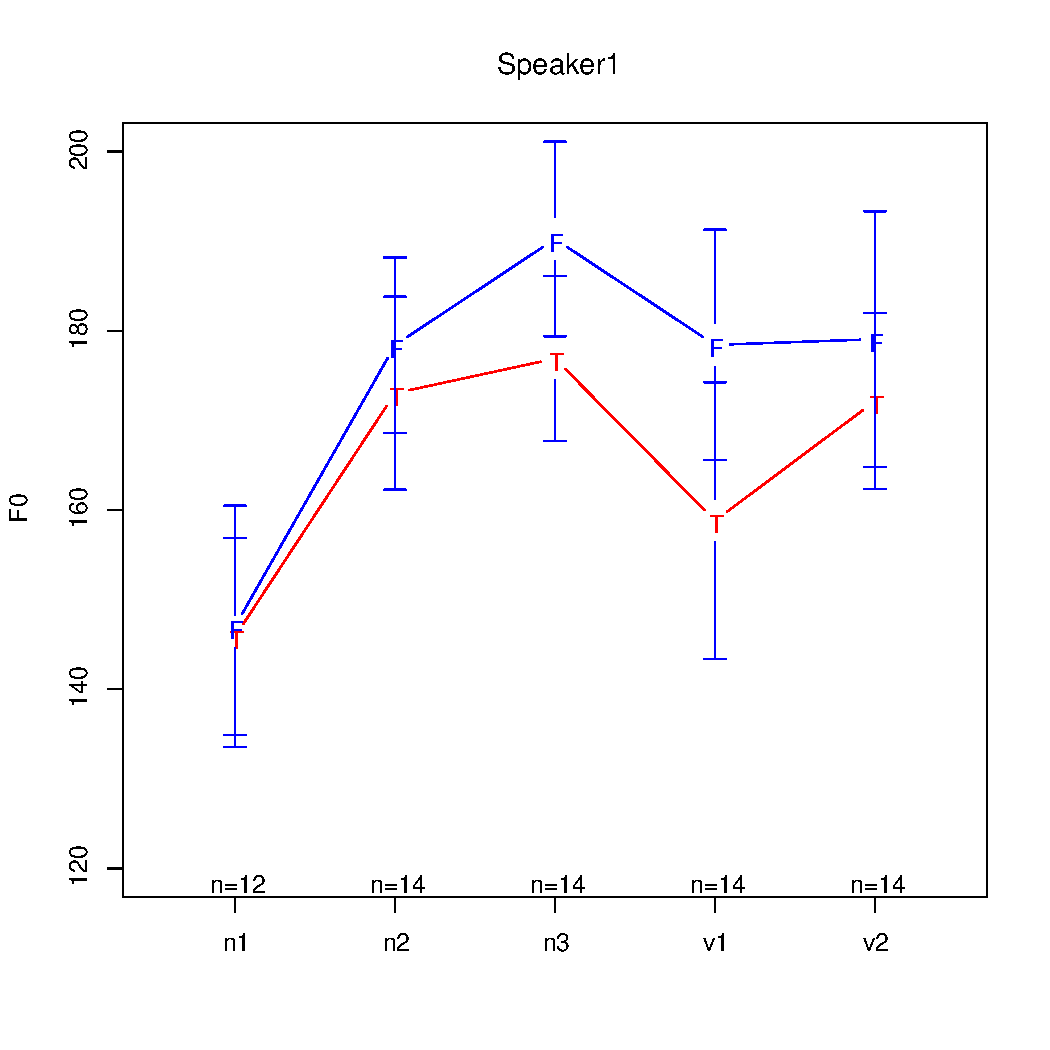
\includegraphics[width=.5\textwidth]{figure/yomiage01.pdf}
	\caption{F$_{0}$ of vowels (Speaker 1)}
	\label{Int:fig:Sp1}
	\end{center}
%\end{minipage}
\end{figure}
\begin{figure}
%\begin{minipage}{0.5\textwidth}
	\begin{center}
	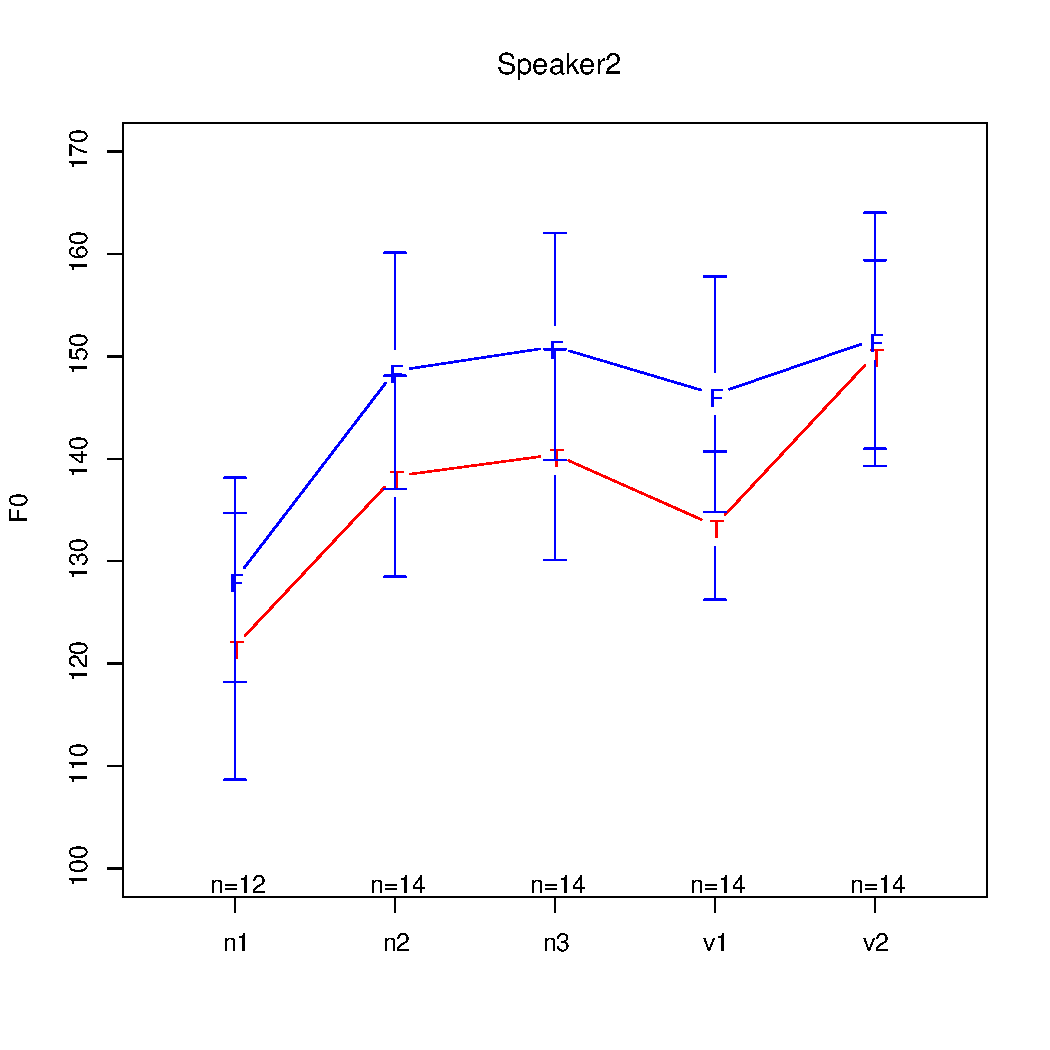
\includegraphics[width=.5\textwidth]{figure/yomiage02.pdf}
	\caption{F$_{0}$ of vowels (Speaker 2)}
	\label{Int:fig:Sp2}
	\end{center}
%\end{minipage}
\end{figure}
\begin{figure}
%\begin{minipage}{0.5\textwidth}
	\begin{center}
	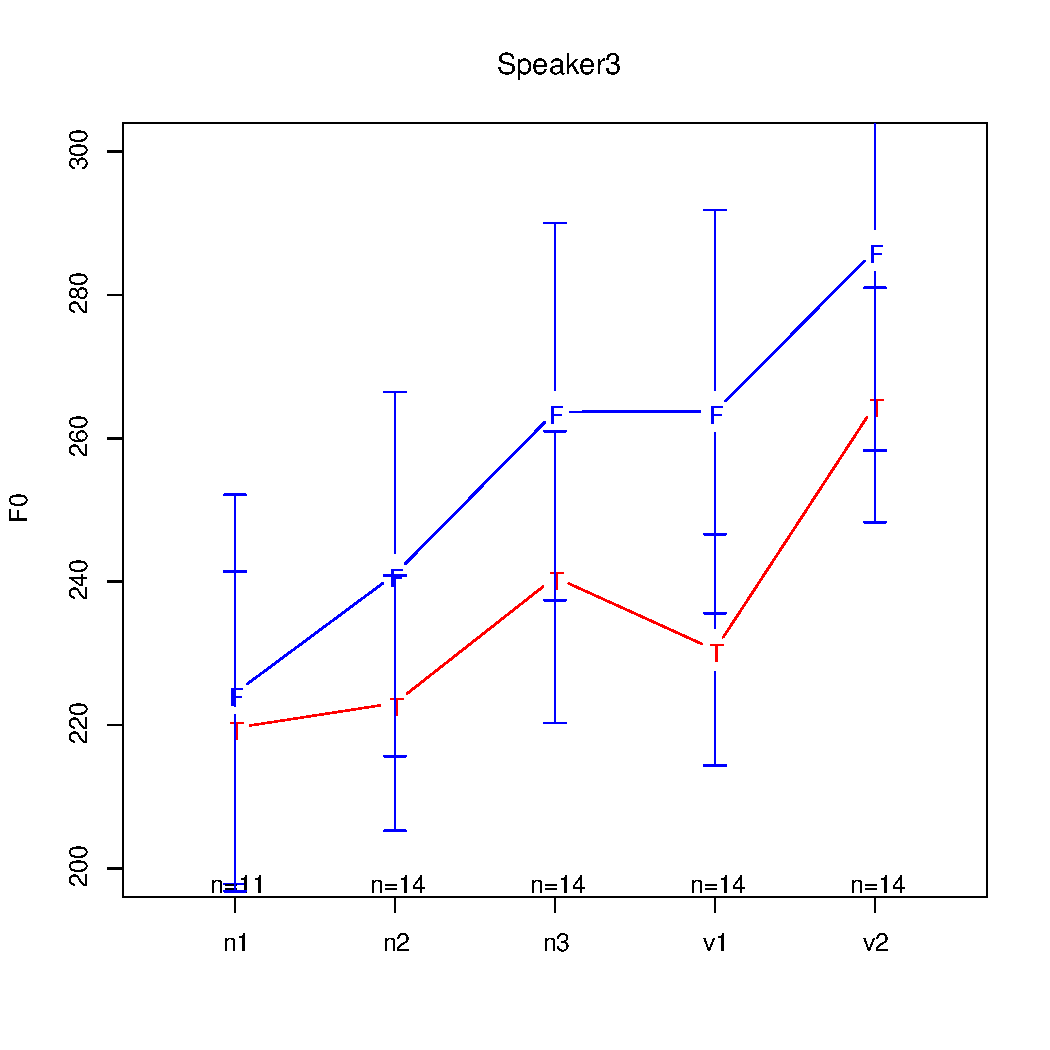
\includegraphics[width=.5\textwidth]{figure/yomiage03.pdf}
	\caption{F$_{0}$ of vowels (Speaker 3)}
	\label{Int:fig:Sp3}
	\end{center}
%\end{minipage}
\end{figure}
\begin{figure}
%\begin{minipage}{0.5\textwidth}
	\begin{center}
	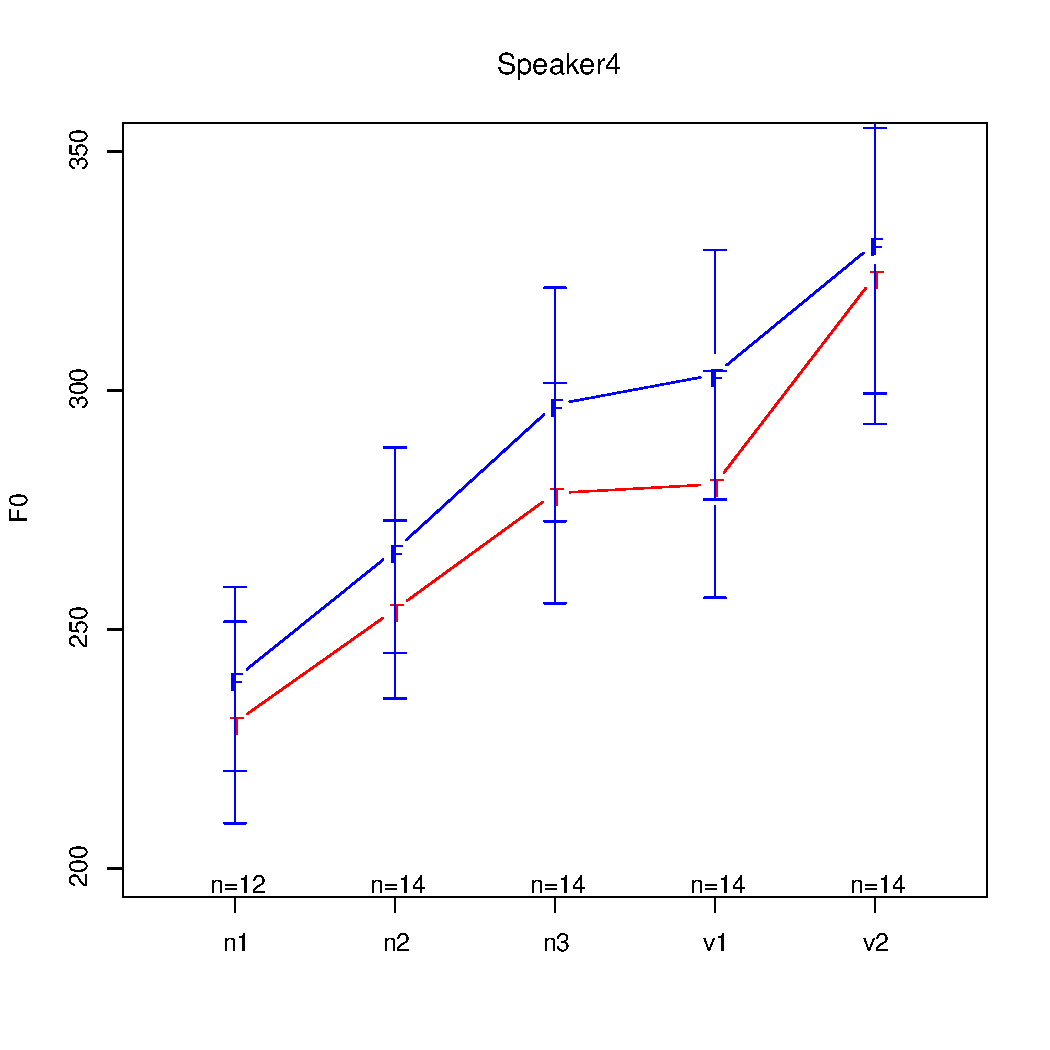
\includegraphics[width=.5\textwidth]{figure/yomiage04.pdf}
	\caption{F$_{0}$ of vowels (Speaker 4)}
	\label{Int:fig:Sp4}
	\end{center}
%\end{minipage}
\end{figure}

%\begin{figure}
%\begin{minipage}{0.5\textwidth}
%	\begin{center}
%	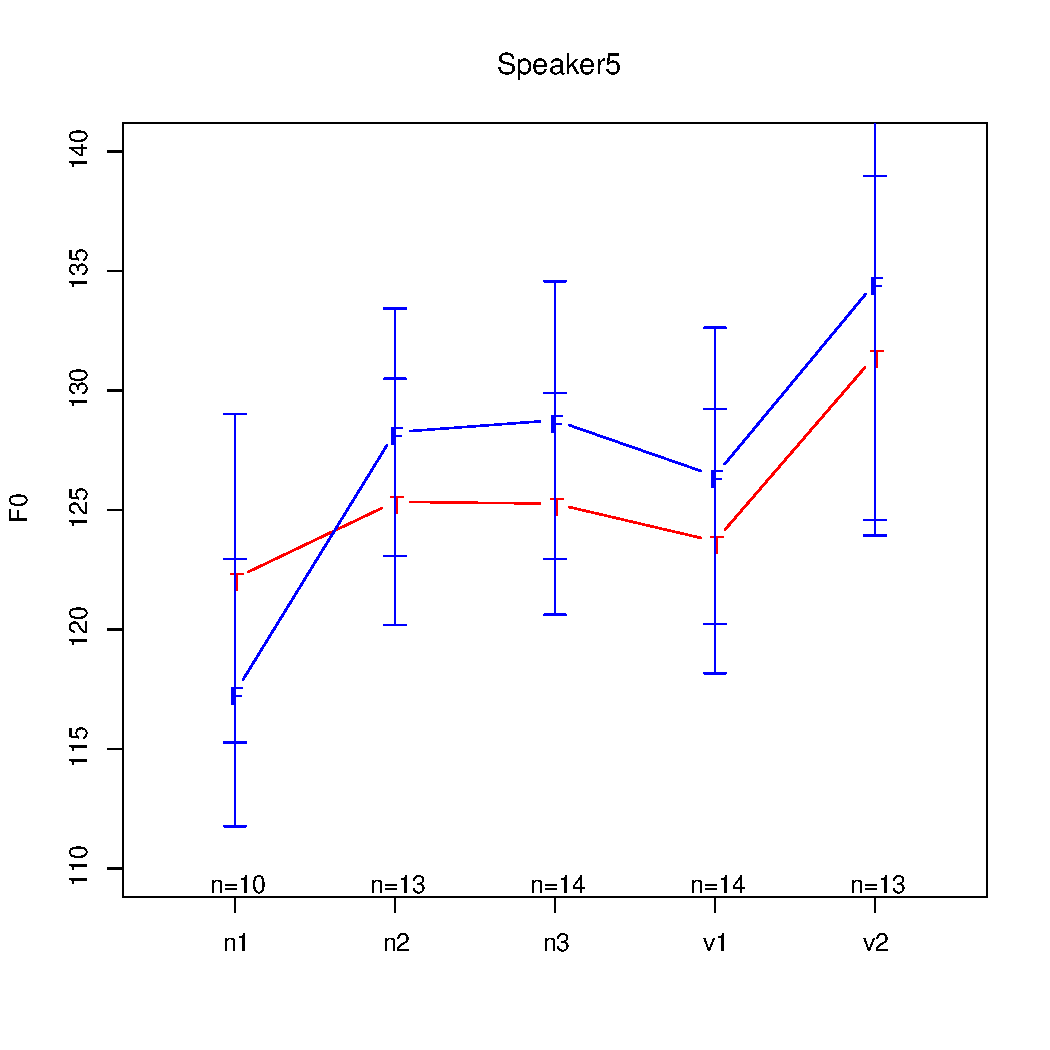
\includegraphics[width=.95\textwidth]{figure/yomiage05.pdf}
%	\end{center}
%\end{minipage}
%\begin{minipage}{0.5\textwidth}
%	\begin{center}
%	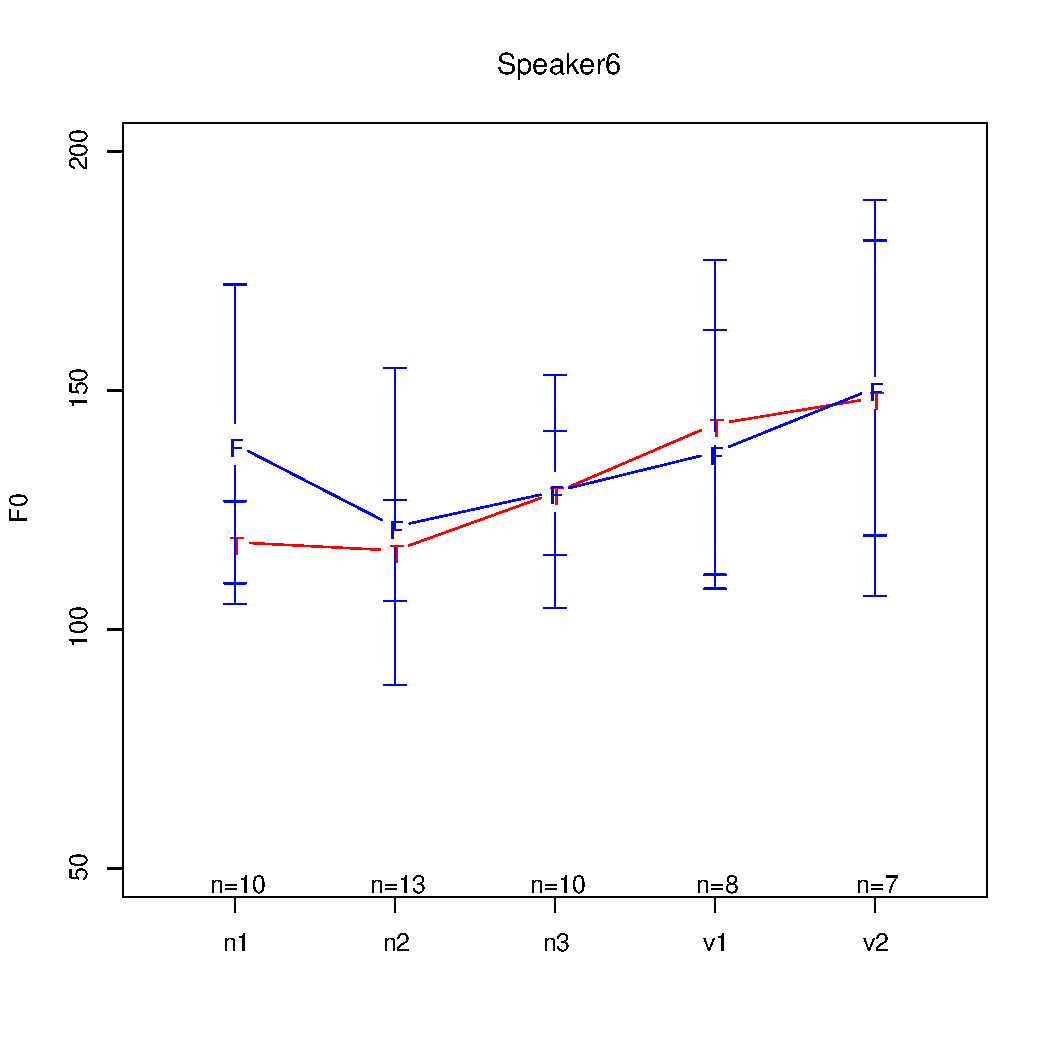
\includegraphics[width=.95\textwidth]{figure/yomiage06.pdf}
%	\end{center}
%\end{minipage}
%\begin{minipage}{0.5\textwidth}
%	\begin{center}
%	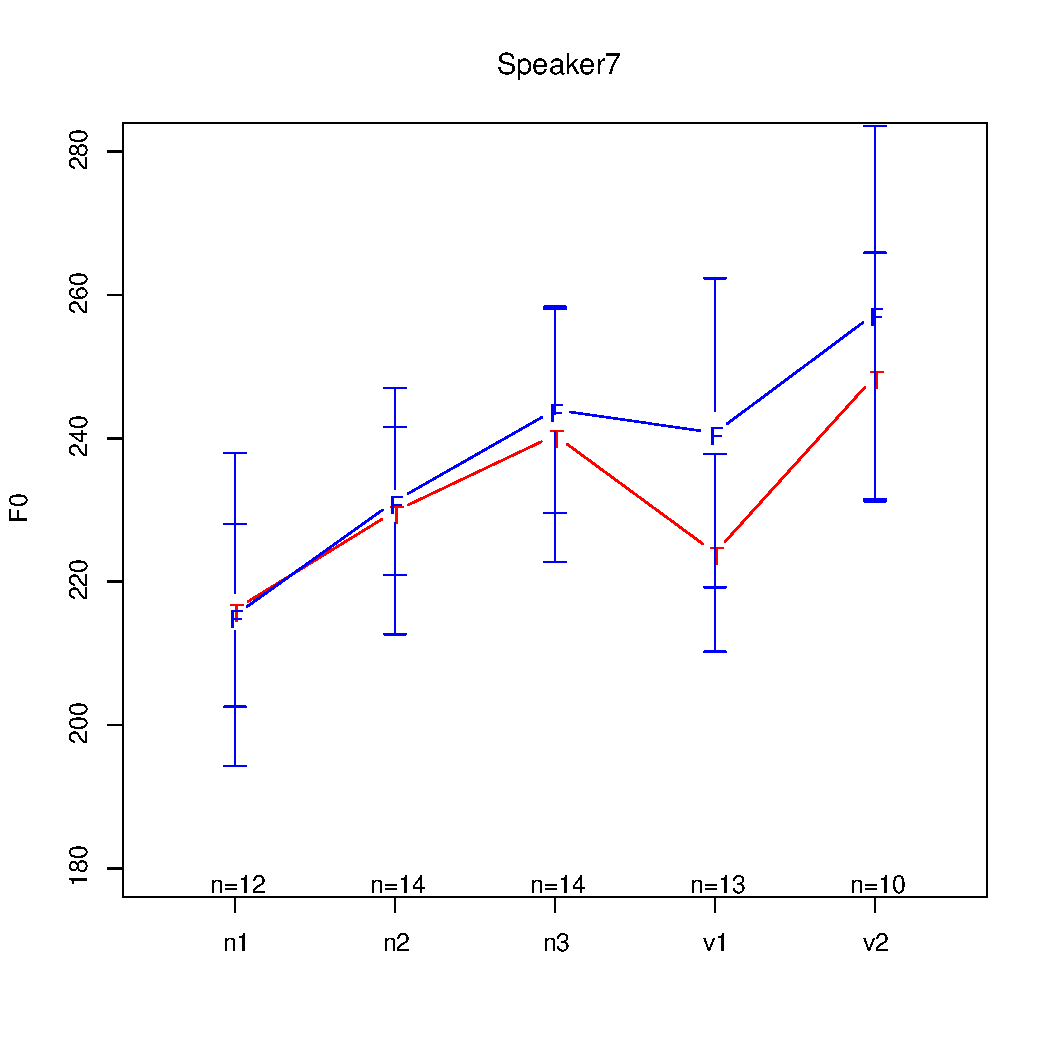
\includegraphics[width=.95\textwidth]{figure/yomiage07.pdf}
%	\end{center}
%\end{minipage}
%\end{figure}

A logistic regression analysis supports this impression.
Table \ref{Pitchv1n3GlmT} and \ref{Pitchv2v1GlmT} show the results of the regression analysis.
The dependent value is the F$_{0}$ difference between the adjacent morae of each \isi{utterance};
in Table \ref{Pitchv1n3GlmT}, the dependent value is the F$_{0}$ difference between \code{n3} and \code{v1},
while, in Table \ref{Pitchv2v1GlmT},
it is the difference between \code{v1} and \code{v2}.
The independent values (predictors) are \isi{information structure} (the distinction between the predicate- vs.~all-focus contexts),
\isi{grammatical relation} (the distinction between the subject and the object),
in addition to speakers and items as random effects.

Table \ref{Pitchv1n3GlmT} shows that
the \isi{predicate-focus context} significantly contributes to
the F$_{0}$ difference between \code{n3} and \code{v1}.
The fact that the estimate is minus indicates that the F$_{0}$ value of \code{v1} is lower than that of \code{n3},
which leads to the conclusion that there is a \isi{pitch reset} in \code{v1}.
Table \ref{Pitchv2v1GlmT} shows that, on the other hand,
both the \isi{predicate-focus structure} as well as the subject significantly contribute to the F$_{0}$ difference between \code{v1} and \code{v2}.
The estimate is plus this time,
which indicates that there is a \isi{pitch} rising from \code{v1} to \code{v2}.%
	\footnote{I do not have an explanation why the subject also contributes to the \isi{pitch} difference of verbs.
	Further investigation is definitely necessary.}
To summarize,
there is a \isi{pitch reset} in the \isi{first mora} of the \isi{verb} in the \isi{predicate-focus context}, where the noun is \isi{topic},
while the \isi{pitch reset} is not observed in the all-focus context.


\begin{table}
%\begin{minipage}{0.9\textwidth}
\centering
\caption{Results of logistic regression analysis (\code{v1-n3})}
\begin{tabular}{lrrr}
\toprule
Coefficients  & Estimate & p-value & \\
\midrule
 Information structure (predicate-focus)          & $-5.591$   & $0.0437$  & *  \\
 Grammatical relation (subject)          & $0.7901$   & $0.7758$  &   \\
\bottomrule
\end{tabular} \\
%\hfill{(0 $\le$ `***' $\le$ 0.001 $\le$ `**' $\le$ 0.01 $\le$ `*' $\le$ 0.05 `.' $\le$ 0.1 $\le$ ` ' 1)}
\label{Pitchv1n3GlmT}
%\end{minipage}
\end{table}

\begin{table}
%\begin{minipage}{0.9\textwidth}
\centering
\caption{Results of logistic regression analysis (\code{v2-v1})}
\begin{tabular}{lrrr}
\toprule
Coefficients  & Estimate & p-value & \\
\midrule
 Information structure (predicate-focus)    & $8.5667$   & $0.0149$  & *  \\
 Grammatical relation (subject)     & $8.2356$   & $0.0221$  & *  \\
\bottomrule
\end{tabular} \\
\hfill{(0 $\le$ `***' $\le$ 0.001 $\le$ `**' $\le$ 0.01 $\le$ `*' $\le$ 0.05 `.' $\le$ 0.1 $\le$ ` ' 1)}
\label{Pitchv2v1GlmT}
%\end{minipage}
\end{table}

Examples of the \isi{pitch} contours of actual production are shown
in Figure \ref{Int:Fig:koinut} and \ref{Int:Fig:koinuf}.
In Figure \ref{Int:Fig:koinut},
where one of the participants of the experiment uttered \ref{koinut},
there is a \isi{pitch reset} in the \isi{first mora} of the \isi{verb} \ci{yuzut-ta} `gave',
while in Figure \ref{Int:Fig:koinuf},
where the same participant uttered \ref{koinuf},
there is no \isi{pitch reset}.

\begin{figure}
%\begin{minipage}{0.5\textwidth}
	\begin{center}
		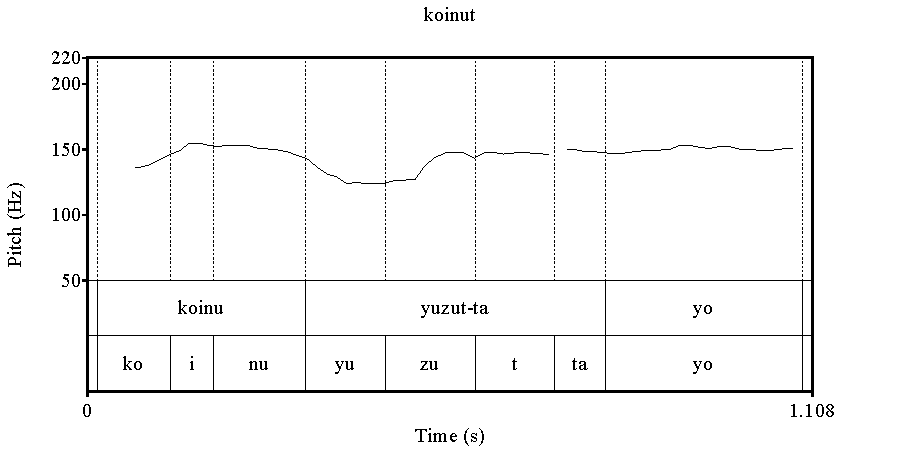
\includegraphics[width=.6\textwidth]{figure/pitcht.pdf}
	\end{center}
	\caption{Pitch contour of \ref{koinut}}
	\label{Int:Fig:koinut}
%\end{minipage}
\end{figure}
\begin{figure}
%\begin{minipage}{0.5\textwidth}
	\begin{center}
		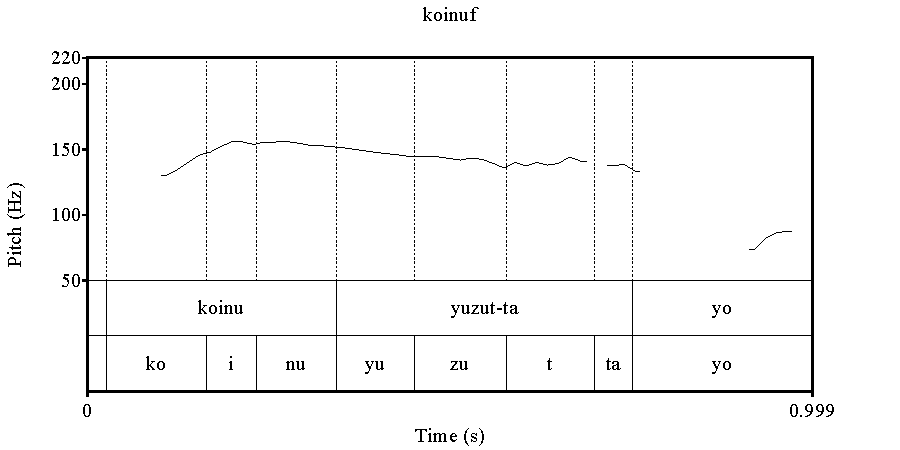
\includegraphics[width=.6\textwidth]{figure/pitchf.pdf}
	\end{center}
	\caption{Pitch contour of \ref{koinuf}}
	\label{Int:Fig:koinuf}
%\end{minipage}
\end{figure}

I also measured the \isi{vowel} length of the last mora of the nouns.
However, neither \isi{information structure} nor \isi{grammatical relation} significantly contributes to the \isi{vowel} length.
In addition, I conducted the regression analysis
using the pitch-range difference between the noun and the \isi{verb} as a dependent variable.
Again, however,
neither \isi{information structure} nor \isi{grammatical relation} significantly contribute to the pitch-range difference.


%%%----------------------------------------------------
%\subsection{Discussion}
%
%These results suggest that
%the \isi{pitch reset} depends on \isi{information structure} and
%\isi{word order} or \isi{topic} marking is independent of intonation.
%It also indicates that the \isi{pitch reset}
%is more important factor for a unit of \isi{information structure}
%rather than the \isi{vowel} length and the \isi{pitch range},
%as I suggested in \S \ref{Int:Cor:Topic:CIU} and \S \ref{Int:Cor:Focus:PIU}.
%
%I argue that phrase-final \isi{pitch} movements are also important factor for \isi{information structure}.
%The phrase final particles such as \ci{ne} and \ci{sa}, with rapid rising or falling \isi{pitch} (i.e., boundary \isi{pitch} movements), can be attached to \isi{topic} NPs, but not to focus NPs.
%In \Next and \NNext, for example,
%assuming that the preceding contexts are the same as (\ref{koinut}) and (\ref{koinuf}) respectively,
%the \isi{topic} \ci{koinu} `puppy' can be attached to \ci{ne} and \ci{sa},
%while the focus \ci{koinu} `puppy' cannot felicitously attached to these particles.
%%
%\ex.\tl{Predicate-focus context}
% \ag.[] sooieba [koinu-\{\EM{ne\tp{:}}/\EM{sa\tp{:}}\}]$_{T}$ [yuzut-ta-yo]$_{F}$ \\
%		by.the.way puppy-\ab{fp} give-\ab{past}-\ab{fp} \\
%		`By the way, (I) gave the puppy (to somebody).'
%
%\ex.\tl{All-focus context}
%	\ag.[] ??kinoo-wa [koinu-\{\EM{ne\tp{:}}/\EM{sa\tp{:}}\} yuzut-ta-yo]$_{F}$ \\
%			yesterday-\ci{wa}-\ab{fp} puppy give-\ab{past}-\ab{fp} \\
%			`Yesterday (we) gave puppies.'
%
%The particles such as \ci{ne} and \ci{sa} are typically uttered in 
%rapid rising or falling \isi{pitch},
%as shown in Figure \ref{Int:Fig:koinune1} and \ref{Int:Fig:koinune2} (the author's speech).
%
%This kind of boundary \isi{pitch} movement is impossible without particles such as \ci{wa}, \ci{ga}, \ci{o}, \ci{ne}, and \ci{sa}
%because in Japanese it is necessary to produce content words with the specified lexical \isi{pitch} pattern.
%%%% 先行研究を追加
%
%%Fillers, sentence initial elements and \isi{topic} markers tend to be lengthened in a long \isi{utterance} \cite{watanabeden10}.
%
%\begin{figure}
%\begin{minipage}{0.5\textwidth}
%	\begin{center}
%		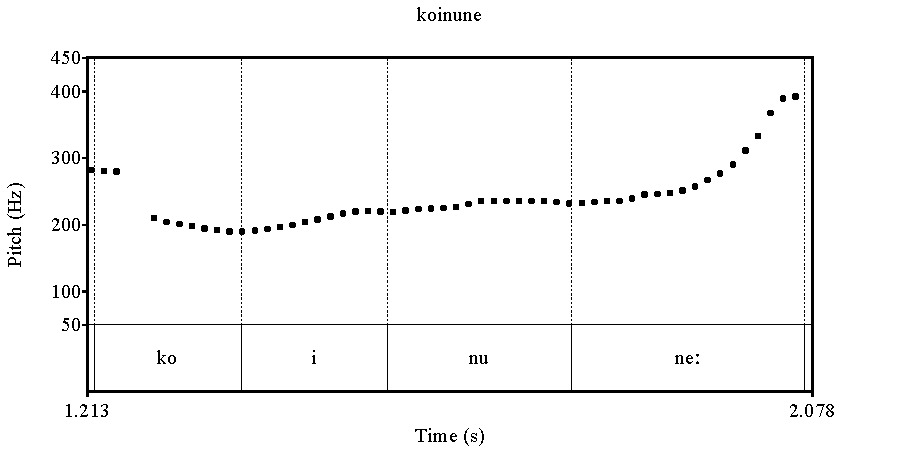
\includegraphics[width=.95\textwidth]{sounds/koinune1.pdf}
%	\end{center}
%	\caption{Pitch contour of \ci{koinu ne} with rapid rising}
%	\label{Int:Fig:koinune1}
%\end{minipage}
%\begin{minipage}{0.5\textwidth}
%	\begin{center}
%		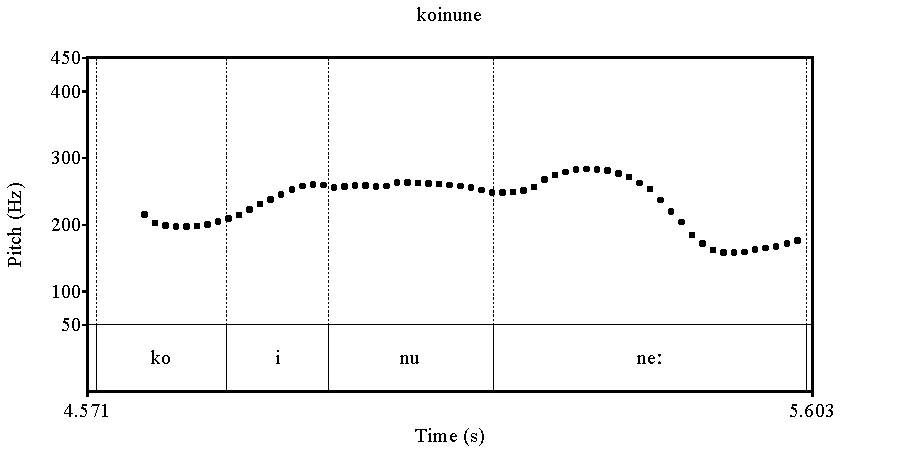
\includegraphics[width=.95\textwidth]{sounds/koinune2.pdf}
%	\end{center}
%	\caption{Pitch contour of \ci{koinu ne} with falling}
%	\label{Int:Fig:koinune2}
%\end{minipage}
%\end{figure}
%%\begin{figure}
%%\begin{minipage}{0.5\textwidth}
%%	\begin{center}
%%		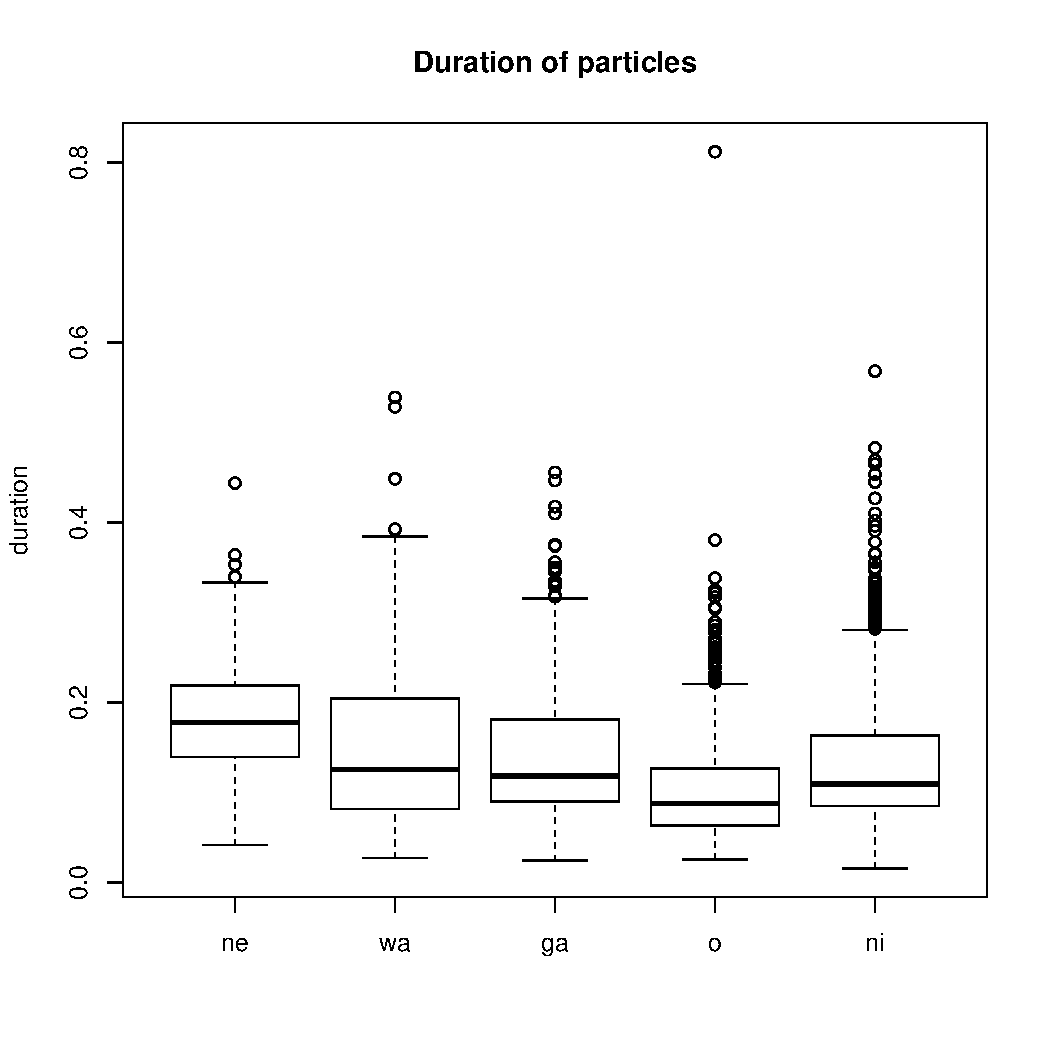
\includegraphics[width=.95\textwidth]{figure/PartLength.pdf}
%%	\end{center}
%%	\caption{}
%%	\label{Int:Fig:PartLength}
%%\end{minipage}
%%\begin{minipage}{0.5\textwidth}
%%	\begin{center}
%%		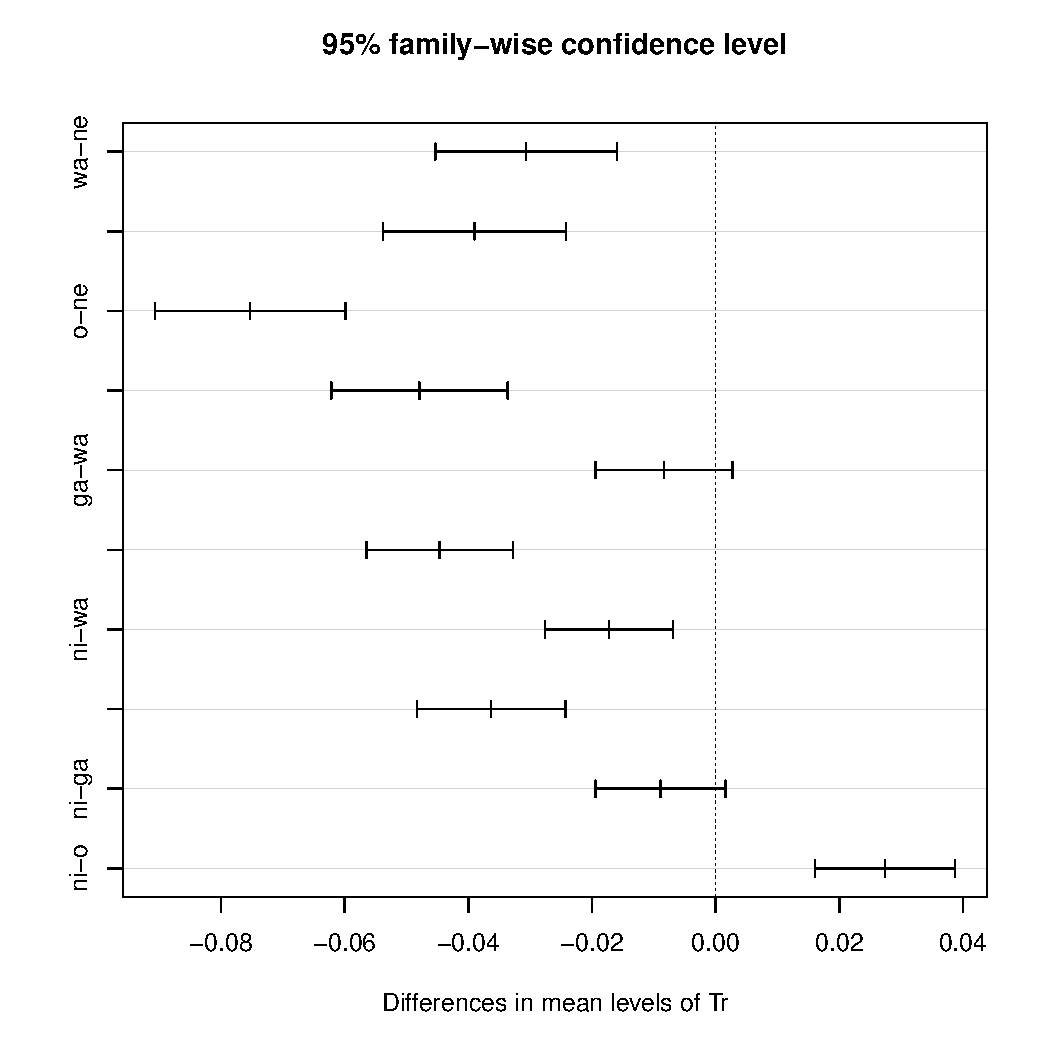
\includegraphics[width=.95\textwidth]{figure/PartLengthTukey.pdf}
%%	\end{center}
%%	\caption{}
%%	\label{Int:Fig:PartLengthTukey}
%%\end{minipage}
%%\end{figure}

%%----------------------------------------------------
\subsection{Summary of experimental study}

In this section,
I discussed the results of the \isi{production experiment}
and concluded that
\isi{topic} elements are produced intonationally separated from the focus predicate,
namely, in phrasal IUs;
while elements which consist of focus with the predicate are produced intonationally unified with the predicate,
namely, in \isi{clausal} IUs.


%%----------------------------------------------------
%%----------------------------------------------------
\section{Discussion}\label{Int:Disc}

This section discusses motivations for intonation units.

%%----------------------------------------------------
\subsection{Principles of intonation unit, information structure, and activation cost}

I propose two closely related motivations for evoked, \isi{inferable}, declining, and unused topics in phrasal IUs and for foci in \isi{clausal} IUs.
First,
uttering an evoked, \isi{inferable}, declining, or unused \isi{topic}, typically a noun followed by a \isi{topic} particle, in an IU and
a focus, typically the predicate and optionally a noun, in another IU
is iconic and easy to process for both the speaker and the \isi{hearer}.
I call it the iconic principle of \isi{intonation unit} and \isi{information structure} \Next.
%
\ex.\label{IUIconicP}\tl{The iconic principle of \isi{intonation unit} and information structure}:
	In spoken language,
	an IU tends to correspond to a unit of \isi{information structure}.

This motivates the tendency that
an evoked \isi{topic} tends to be uttered in a phrasal IU and
a focus uttered in a \isi{clausal} IU.

Second,
strongly evoked elements are proposed to be produced in a coherent IU with the predicate,
namely, in a \isi{clausal} IU;
elements with \isi{low activation cost} are not produced by themselves.
Based on this observation,
I propose the principle of IU and \isi{activation cost}.
%
\ex.\label{IUActCostP}\tl{The principle of \isi{intonation unit} and activation cost}:
     all substantive IUs have similar activation costs;
     there are few IUs with only a strongly evoked element or
     those with too much new elements.

This is inspired by, but also elaborates, ``one new idea at a time'' constraint in \citeA{chafe87,chafe94}.
\citeA{chafe87,chafe94}, and \citeA{matsumoto03}, who follows Chafe,
considers this ``one idea'' corresponds to a grammatical category such as subject, object, and \isi{verb}.
\citeA[p.~110 ff.]{chafe94}, for example, discusses IUs consisting of an object and a \isi{verb} as exceptional IUs.
He argues that,
in such IUs,
there are special reasons for an object and a \isi{verb} to be produced in an IU;
verbs have been already evoked,
the IU includes a low-content \isi{verb} (such as ``\ci{have, get, give, do, make, take, use} and \ci{say}'', p.~111), or
the object and \isi{verb} is a lexicalized phrase (such as \ci{wash dishes}).
However, in my corpus,
IUs with an object and a \isi{verb} (or a subject and a \isi{verb}) which do not apply
to these conditions are not rare.
For example,
\ci{toti-o uba-u} `deprive (somebody) of land'
is produced in a single IU.
However, the expression is not frequently used in everyday life
and the predicate \ci{uba-u} `deprive' is mentioned for the first time in this \isi{monologue}.
The \isi{verb} \ci{uba-u} `deprive' is not low-content, either.
%
\exg. wareware-no {\iub} \EM{toti-o} \EMi{ubat}-te {\iub} \\
      \ab{1}\ab{pl}-\ab{gen} {} land-\ci{o} deprive-and {} \\
      `(They) deprived our land...'
      \src{S00M0199: 473.79-475.65}
%S00M0199|00473792L|473.792039|489.768786|L|それで(0.106)我々の土地を奪って(0.398)聖地を(D だ)(0.118)(D うばっ)(0.164)(F えー)蹂躙してるということに対して(0.127)聖地を奪還したいという(0.448)(F えー)(F ま)(0.11)同じ国内の民族アルバニア人の(0.132)(F えー)悲願が(0.582)(F えー)ここに来て(0.263)(F えー)(0.888)達成されたいと(0.285)いうことで|<並列節デ>|直後がまとめ表現

Similarly, in \Next[b],
\ci{i-nai kata-ga nana-wari} `those who are absent consist of 70\%'
is neither conventionalized nor evoked,
but it is still produced in a single IU.
%
\ex.
% \ag. hiraki-naoru kata-ga ee soo-su-ne san-wari \\
%      open-correct person-\ab{nom} \ab{fl} so-\ab{cop}.\ab{plt}-\ab{fp} three-ratio \\
%      `Those who '
 \a. Those who do not pay back their debt consist of 30 \%.
 \bg. sorekara {\iub} \EM{i-nai} \EM{kata-ga} \EMi{nana-wari}-to {\iub} \\
      then {} exist-\ab{neg} person-\ci{ga} seven-ratio-\ab{quot} {} \\
      `And, those who are absent consist of 70\%.'
 \b.[] \src{S00M0221: 348.22-356.07}
%S00M0221|00345065L|345.065284|352.276062|L|行ってもですね(0.414)ないものはないっていう形で開き直る方が(1.278)(F えー)そうすね三割||体言止
%S00M0221|00354106L|354.106425|356.073046|L|それからいない方が七割と||体言止

I argue that the NP and the \isi{verb} are produced in a \isi{clausal} IU
because they consist of a unit of \isi{information structure}: focus.
\chd{At the same time, they form a syntactic constituent: VP.}
A unit of focus can contain several clauses through clause-chaining,
but they are usually not realized as a single IU, but as several IUs
because of the limitation of processing,
which is captured by the principle \ref{IUActCostP}.

The principles \ref{IUIconicP} and \ref{IUActCostP} compete with each other and form an actual IU.



%%----------------------------------------------------
\subsection{Principle of the separation of reference and role}

%%%----------------------------------------------------
%\subsubsection{Word order and IU of focal elements}
%
%
%Word order and the distinction between phrasal vs.~\isi{clausal} IUs are interrelated with each other.
%More specifically,
%the information-structure \isi{continuity principle} (\ref{IScontinuityP}) proposed in Chapter \ref{WordOrder},
%repeated here as (\ref{IScontinuityP3}),
%predicts that focus elements (typically P and (patient) S) tend to appear close to the predicate.
%%
%\ex. \label{IScontinuityP3}\tl{Information-structure continuity principle}:
% A unit of \isi{information structure} must be continuous in a clause;
% i.e., elements which belong to the same unit are adjacent with each other.
%
%Also, in the previous sections,
%I claimed that focus elements tend to appear in \isi{clausal} IUs.
%%because of the iconic principle of \isi{intonation unit} and \isi{information structure} (\ref{IUIconicP}).
%Some readers might argue that this result is a natural consequence of the information-structure \isi{continuity principle} (\ref{IScontinuityP3})
%because the elements closer to the predicate are more likely to be \isi{clausal} IUs.
%%However, note that, according to Table \ref{IntonationGlmT},
%%P and S are variables significantly contributing to predicting \isi{clausal} IUs,
%%\EMt{controlling} \isi{word order},
%%i.e., P and S are significant predictors independent of \isi{word order}.
%
%Of course the information-structure \isi{continuity principle} and
%the iconic principle of \isi{intonation unit} and \isi{information structure}
%are two different perspectives of the same thing:
%the tendency of human mind processing.
%A cognitively substantial unit of \isi{information structure} such as \isi{topic} and focus provides motivations for the speaker to utter the \isi{topic} and focus adjacent with each other in a single processing unit.
%Therefore, one cannot tease apart these two.

%%%----------------------------------------------------
%\subsubsection{Clause-chaining and intonation unit}
%
%The same argument also applies to \isi{topic};
%topics tend to be uttered clause-initially in phrasal IUs.
%Word order and the distinction between phrasal vs.~\isi{clausal} IUs
%are closely interrelated with each other and it is impossible to tease them apart because they are motivated by the same tendency of human cognition.
%
%As in Chapter \ref{WordOrder},
%there is a tendency that \isi{topic} (especially) definite elements tend to appear clause-initially.
%The fact that \isi{word order} is a better predictor than \isi{information status} and persistence
%indicates that my way of coding \isi{information status} does not perfectly reflect the status of the element in question,
%rather, \isi{word order} better reflects the status of the referent.
%
%Moreover, as also discussed in Chapter \ref{WordOrder},
%persistent elements tend to appear word-initially and expected to be uttered in phrasal IUs rather than \isi{clausal} IUs.
%However, Table \ref{IntonationGlmT} shows exactly an opposite result;
%persistence is a predictor contributing to \isi{clausal} IUs,
%although this is only marginally significant.
%I believe that this is also because persistence (being persistent) and \isi{word order} (appearing clause-initially) are correlating with each other and \isi{word order} better predicts the distinction between phrasal vs.~\isi{clausal} distinction.
%Persistence and topic-coding is also correlating with each other and, again, topic-coding is a better predictor.
%The remaining examples of persistent elements are exceptional cases such as (\ref{WO:Ex:miss}) and (\ref{WO:Ex:kuruma}) in Chapter \ref{WordOrder}
%where the elements neither are coded by \isi{topic} markers nor appear clause-initially.

I argue that intonation units play an important role in clause-chaining.
%I show a few examples where
%persistent elements, coded by topic-markers, appear clause-initially
%and are uttered in phrasal IUs.
%I also argue that this kind of example is cognitively motivated,
%although their significance is overridden by \isi{word order} and \isi{topic} markers in Table \ref{IntonationGlmT}.
As discussed in Chapter \ref{WordOrder},
uttering persistent elements clause-initially (with \isi{topic} markers) is especially useful in clause-chaining languages;
this announces which element becomes zero in the following \isi{utterance}.
This type of clause-initial elements are often uttered in phrasal IUs rather than \isi{clausal} IUs.
For example, in \Next,
\ci{eberesto-kaidoo} `Everest trail' appears clause-initially,
followed by an IU boundary,
and is mentioned three times in the following clauses as indicated by {\O}.%
 \footnote{
 \chd{{\O} is assumed to appear right before the predicate for the purpose of presentation.
 However, this assumption does not affect the analysis here.}
 }
This big chunk of clauses in \Next as a whole consists of a sentence and
each clause is combined through clause-chaining.
%
\ex.
\ag. \EM{kono} \EM{eberesuto-kaidoo-toiuno-wa} {\tp{\dvline}} \\
	this Everest-trail-\ab{quot}-\ci{wa} {} \\
	`{This Everest Trail} is'
\bg. tibetto-to nepaaru-no \tp{\dvline} kooeki-ro-ni-mo nat-te ori-masi-te\tp{\dvline} \\
	Tibet-\ab{com} Nepal-\ab{gen} {} trade-road-\ab{dat}-also become-and \ab{prog}-\ab{plt}-and \\
	`also used for trading  between Tibet and Nepal.'
\cg. ma zissai-wa nihon-de iu-to \tp{\dvline} \\
	\ab{fl} actual-\ci{wa} Japan-\ab{loc} say-\ab{cond} {} \\
	`Say, in Japan for example,'
\dg. \EM{\O} takao-san-mitaina \tp{\dvline} yama-miti-nan-desu-keredomo \tp{\dvline} \\
	{\O} Takao-mountain-like {} mountain-road-\ab{nmlz}-\ab{cop}.\ab{plt}-though {} \\
	`it's like a road in Mt.\ Takao or something.'
\eg. genti-no hito$\sim$bito-nitotte-wa \tp{\dvline} ee \tp{\dvline} \EM{\O} tuusyoo-ro-to \tp{\dvline} iu-yoona \\
	local-\ab{gen} person$\sim$\ab{pl}-for-\ci{wa} {} \ab{fl} {} {\O} trade-road-\ab{quot} {} say-like \\
\bg. insyoo-no \EM{\O} miti-desi-ta \tp{\dvline} \\
	 impression-\ab{gen} {\O} road-\ab{cop}.\ab{plt}-\ab{past} {} \\
 `{it} was a road like trading road for local people.'
 \b.[] \hfill{(\code{S01F0151: 105.73-120.14})}
%このエベレスト街道というのは
%チベットとネパールの交易路にもなっておりまして
%ま実際は日本で言うと
%高尾山みたいな山道なんですけれども
%現地の人々にとってはえー通商路というような印象の道でした (S01F0151: 105.73-120.14)

To schematize,
utterances like \Next are frequently observed.
%
\ex.
 \a. \fbox{Topic} \tp{\dvline}
 \b. \fbox{Clause1} \tp{\dvline}
 \b. \fbox{Clause2} \tp{\dvline}
 \b. \fbox{Clause3} \tp{\dvline}
 \b. ...

First, the \isi{topic} is uttered clause-initially (often coded by \isi{topic} markers) in a phrasal IU.
Then the explanation about the \isi{topic} follows the \isi{topic}.
In other words, expressions like \Last[a] followed by an IU boundary establishes topics to be mentioned in the following \isi{discourse}.

This type of example is small in number per \isi{monologue} because there is only a few topics introduced in each \isi{monologue}.
This blurs the pattern like \Last in simple count of raw numbers like the one shown in Table \ref{IUPerT} and Figure \ref{IUPerF}.
%Similarly, Table \ref{IUInfoStatusT} and Figure \ref{IUInfoStatusF} appear to indicate that \isi{information status} does not affect the distinction between phrasal vs.~\isi{clausal} IUs.
%For now, \isi{topic} and case markers are better predictors.
%However, this does not mean that the pattern does not exist.
%
%
%\begin{figure}
%\begin{minipage}{0.5\textwidth}
%\centering
% \tblcaption{IU vs.~information status}
% \label{IUInfoStatusT}
% \begin{tabular}{lrr}
% \toprule
%             & Anaphoric & Non-\isi{anaphoric} \\
% \midrule
%  Phrasal IU & 501   & 571 \\
%             & \rt{(65.2\%)} & \rt{(59.4\%)} \\
%  Clausal IU & 267   & 391 \\
%             & \rt{(34.8\%)} & \rt{(40.6\%)} \\
% \midrule
%  Sum        & 768   & 962  \\
%             & \rt{(100\%)} & \rt{(100\%)} \\
% \bottomrule
% \end{tabular}
%%        Phrasal Clausal
%%  Anaphoric     501     267
%%  Non-\isi{anaphoric}       571     391
%\end{minipage}
%\begin{minipage}{0.5\textwidth}
%\centering
% \tblcaption{IU vs.~Persistence}
% \label{IUPerT}
% \begin{tabular}{lrr}
% \toprule
%             & Persistent & Non-Persistent \\
% \midrule
%  Phrasal IU & 524        & 548 \\
%             & \rt{(63.2\%)} & \rt{(60.8\%)} \\
%  Clausal IU & 305        & 353 \\
%             & \rt{(36.8\%)} & \rt{(39.2\%)} \\
% \midrule
%  Sum        & 829        & 901  \\
%             & \rt{(100\%)} & \rt{(100\%)} \\
% \bottomrule
% \end{tabular}
%%                 Phrasal Clausal
%%  Persistent         524     305
%%  Non-Persistent     548     353
%\end{minipage}
%
%\begin{minipage}{0.5\textwidth}
%	\begin{center}
%	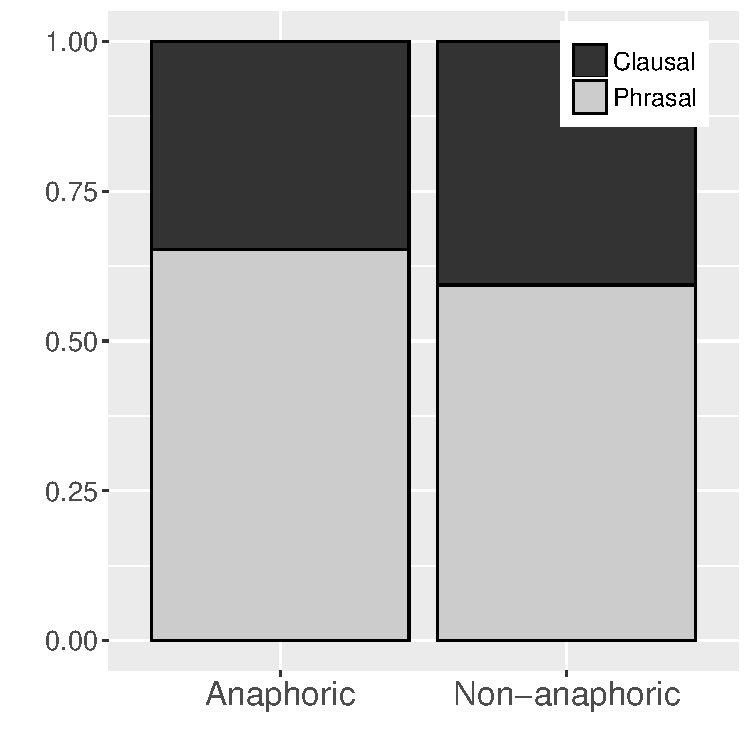
\includegraphics[width=.95\textwidth]{figure/IUInfoStatus.pdf}
%	\caption{IU vs.~information status}
%	\label{IUInfoStatusF}
%	\end{center}
%\end{minipage}
%\begin{minipage}{0.5\textwidth}
%	\begin{center}
%	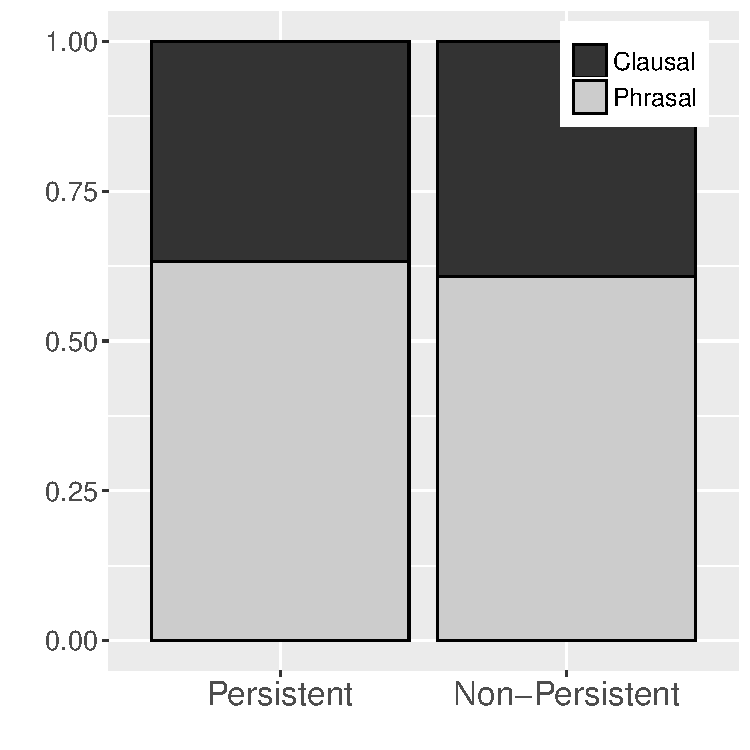
\includegraphics[width=.95\textwidth]{figure/IUPer.pdf}
%	\caption{IU vs.~persistence}
%	\label{IUPerF}
%	\end{center}
%\end{minipage}
%\end{figure}

I argue that the tendency schematized in \Last is a realization
of the principle of the separation of reference and role proposed by
\citeA{lambrecht94}.
\citeA[184-185]{lambrecht94} argues:
``[t]he non-canonical configurations thus allow speakers to separate the {\sc referring} function of noun phrases from the {\sc relational} role their denotata play as arguments in a proposition. [...]
I will call the grammatical principle whereby the lexical representation of a \isi{topic} referent takes place separately from the designation of the referent's role as an argument in a proposition the {\sc principle of the separation of reference and role} (PSRR) for \isi{topic} expressions. The communicative motivation of this principle can be captured in the form of a simple pragmatic maxim:
`Do not introduce a referent and talk about it in the same clause'''.
In Japanese,
PSRR is reflected by the fact that
\isi{topic} elements are also separated intonationally from the clause.


%%----------------------------------------------------
%%----------------------------------------------------
\section{Summary}

%%----------------------------------------------------
\subsection{Summary of this chapter}


This chapter analyzed intonation units in Japanese
in terms of whether an NP is intonationally separated from the predicate or not.
It argued that evoked, \isi{inferable}, declining, and unused topics tend to be separated intonationally from the predicate,
while strongly evoked topics tend to be integrated into the predicate.
On the other hand,
focus elements tend to be integrated into the predicate
to form a unit of focus with the predicate.
I proposed three inter-related principles at work to determine
intonation units in Japanese.



%%----------------------------------------------------
\subsection{Remaining issues}

In this chapter,
I proposed to modify the definitions of intonation units.
Further studies are needed to investigate cognitively-valid definitions of intonation units.
Furthermore, it is also necessary to come up with methodology to find a unit of processing independent of intonation
to avoid circularity.






